\section{Layout of the Gilbert Cell}
The overall layout was carried on in place with a view to:
\begin{itemize}
	\item reducing technology gradients using common centroid, interdigitated or multi-finger structures;
	\item placing components all in the same direction for a uniform error affection;
	\item reducing border effects with dummy elements;
	\item minimizing encroachment errors with same-length transistor fingers;
 	\item limiting substrate noise with guard rings;
	\item avoiding connections which could lead to crosstalk;
	\item minimizing metal changes in the routing process;
	\item aiming a compact structure.
\end{itemize}
\subsection{Differential RF stage}
A careful attention has been paid to the layout of differential pairs like the one of RF stage. Since it's desirable to have the most symmetric input stage a common centroid configuration has been employed, following a structure sketched as in figure \ref{fig:diff_CC}. 

\begin{figure}[H]
	\centering
	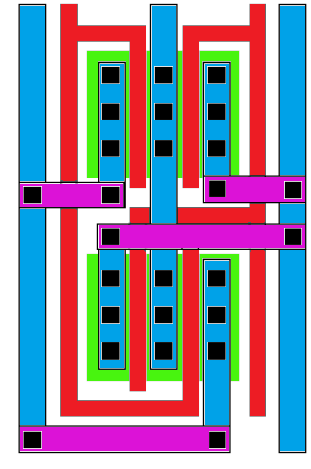
\includegraphics[scale=0.6]{diff_CC}
	\caption{Common centroid structure used for differential RF stage}
	\label{fig:diff_CC}
\end{figure}
This minimizes errors due to process gradients within the planar structure. Dummy elements where also placed next to the four transistors at the edges to guarantee a uniform dopant concentration of the inner transistors.

Dummy MOSFETs' drain and source are tied together and then short circuited to source.
The transistor length of the differential pair has been divided to form multi-finger  transistors, such that the whole structure results as square and compact as possible. This was intended again for the purpose of reducing gradients and with a glance forward to the overall mixer layout's compactness . The final layout of differential RF pair is shown in figure \ref{L_RF_full}.
\begin{figure}[H]
	\centering
	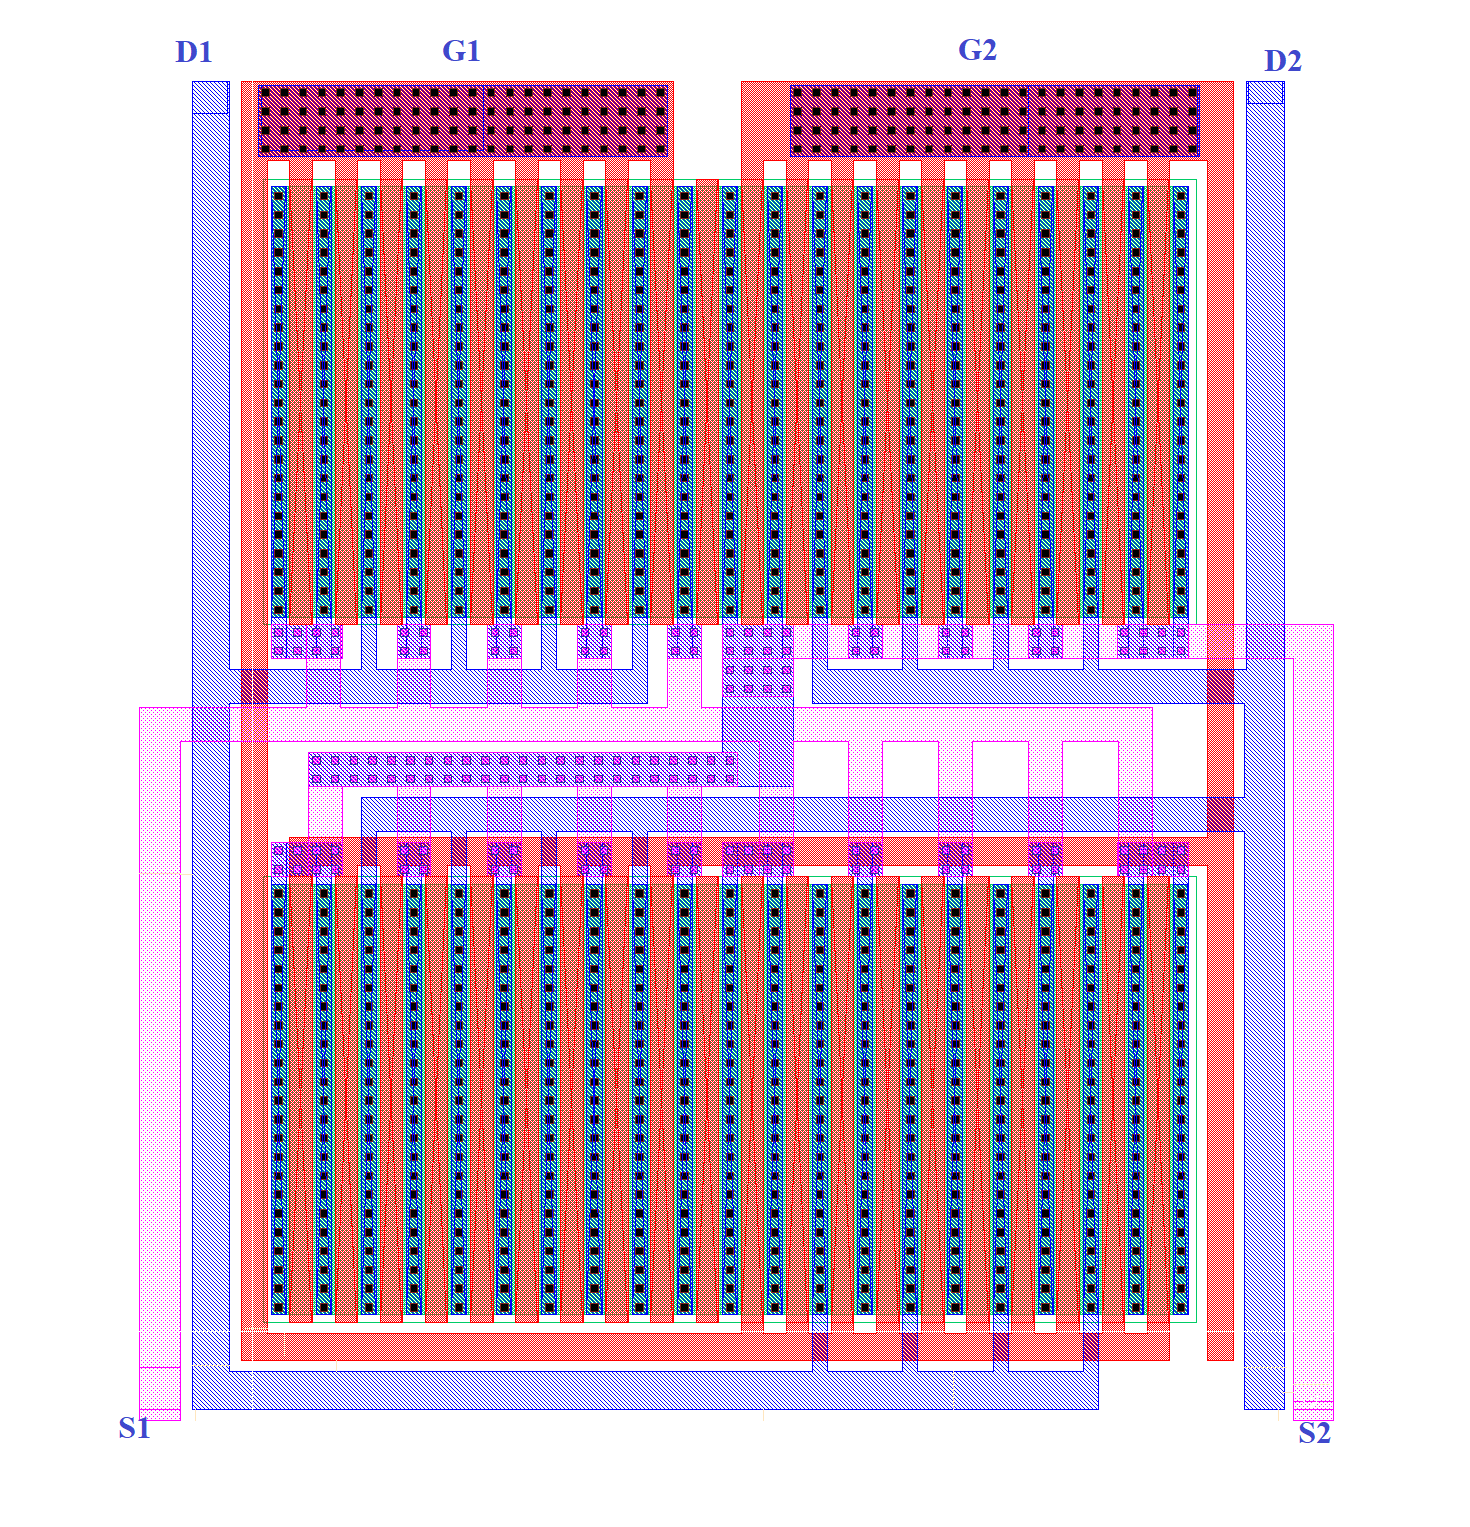
\includegraphics[scale=0.25]{L_RF_full}
	\caption{Complete layout of RF differential transistor}
	\label{L_RF_full}
\end{figure}

\newpage
\subsection{Differential LO stages}
The two differential LO stages have been designed trying to prevent the same mismatch causes seen for the RF stage. Two common centroid structure were drawn at first. Being the transistor wide, multi-finger structure was employed also here to have an almost-square layout along with dummy elements. Attention has been paid in so that the two LO pairs could be easily stack above the RF stage with the same width. 
Secondly, we opted for a merging of the two common centroid LO layouts in a more compact tiled layout. The gate disposal simplifies the access to these nets from the signal capacitors in the global layout. Final LO layout is shown in figure \ref{L_LO_full} .

\begin{figure}[H]
	\centering
	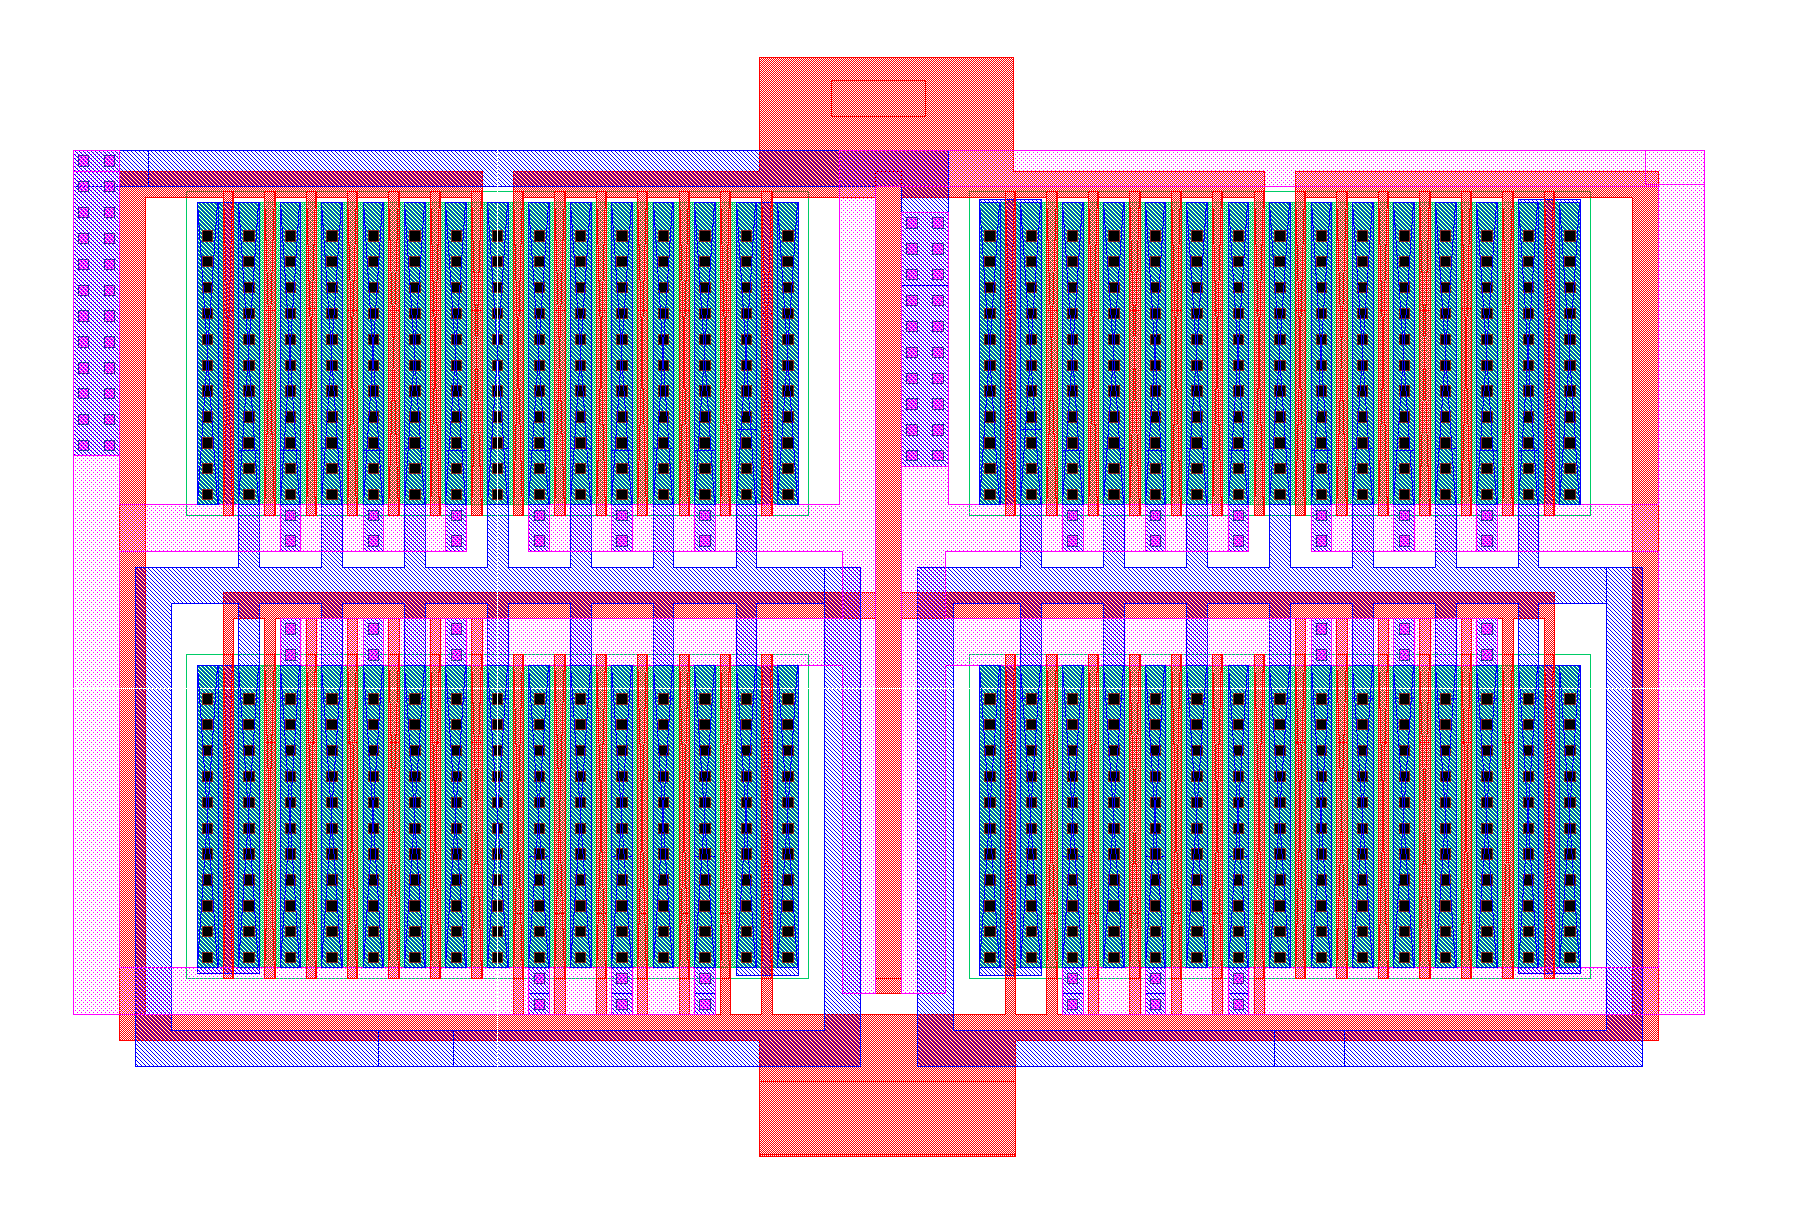
\includegraphics[width=\textwidth]{L_LO_full}
	\caption{Complete layout of LO differential stages}
	\label{L_LO_full}
\end{figure}

\subsection{Current mirror and diode connected transistor}
Current mirror employs an interdigitated structure similar to the one visible in \textbf{figure}.
%\begin{figure}[H]
%	\centering
%	\includegraphics[scale=0.6]{NAME}
%	\caption{CAPTION}
%	\label{LABEL}
%\end{figure}

Since fingers are all the same size the current ratio is independent from encroachment width. Dummy transistors was included to reduce border effects, and source connections on both top and bottom sides have been added for a small source resistance. The weak branch transistor's drain has been tied together to the gate with an array of contacts. The final layout for current mirror is visible in \ref{L_curmir_full}.

\begin{figure}[H]
	\centering
	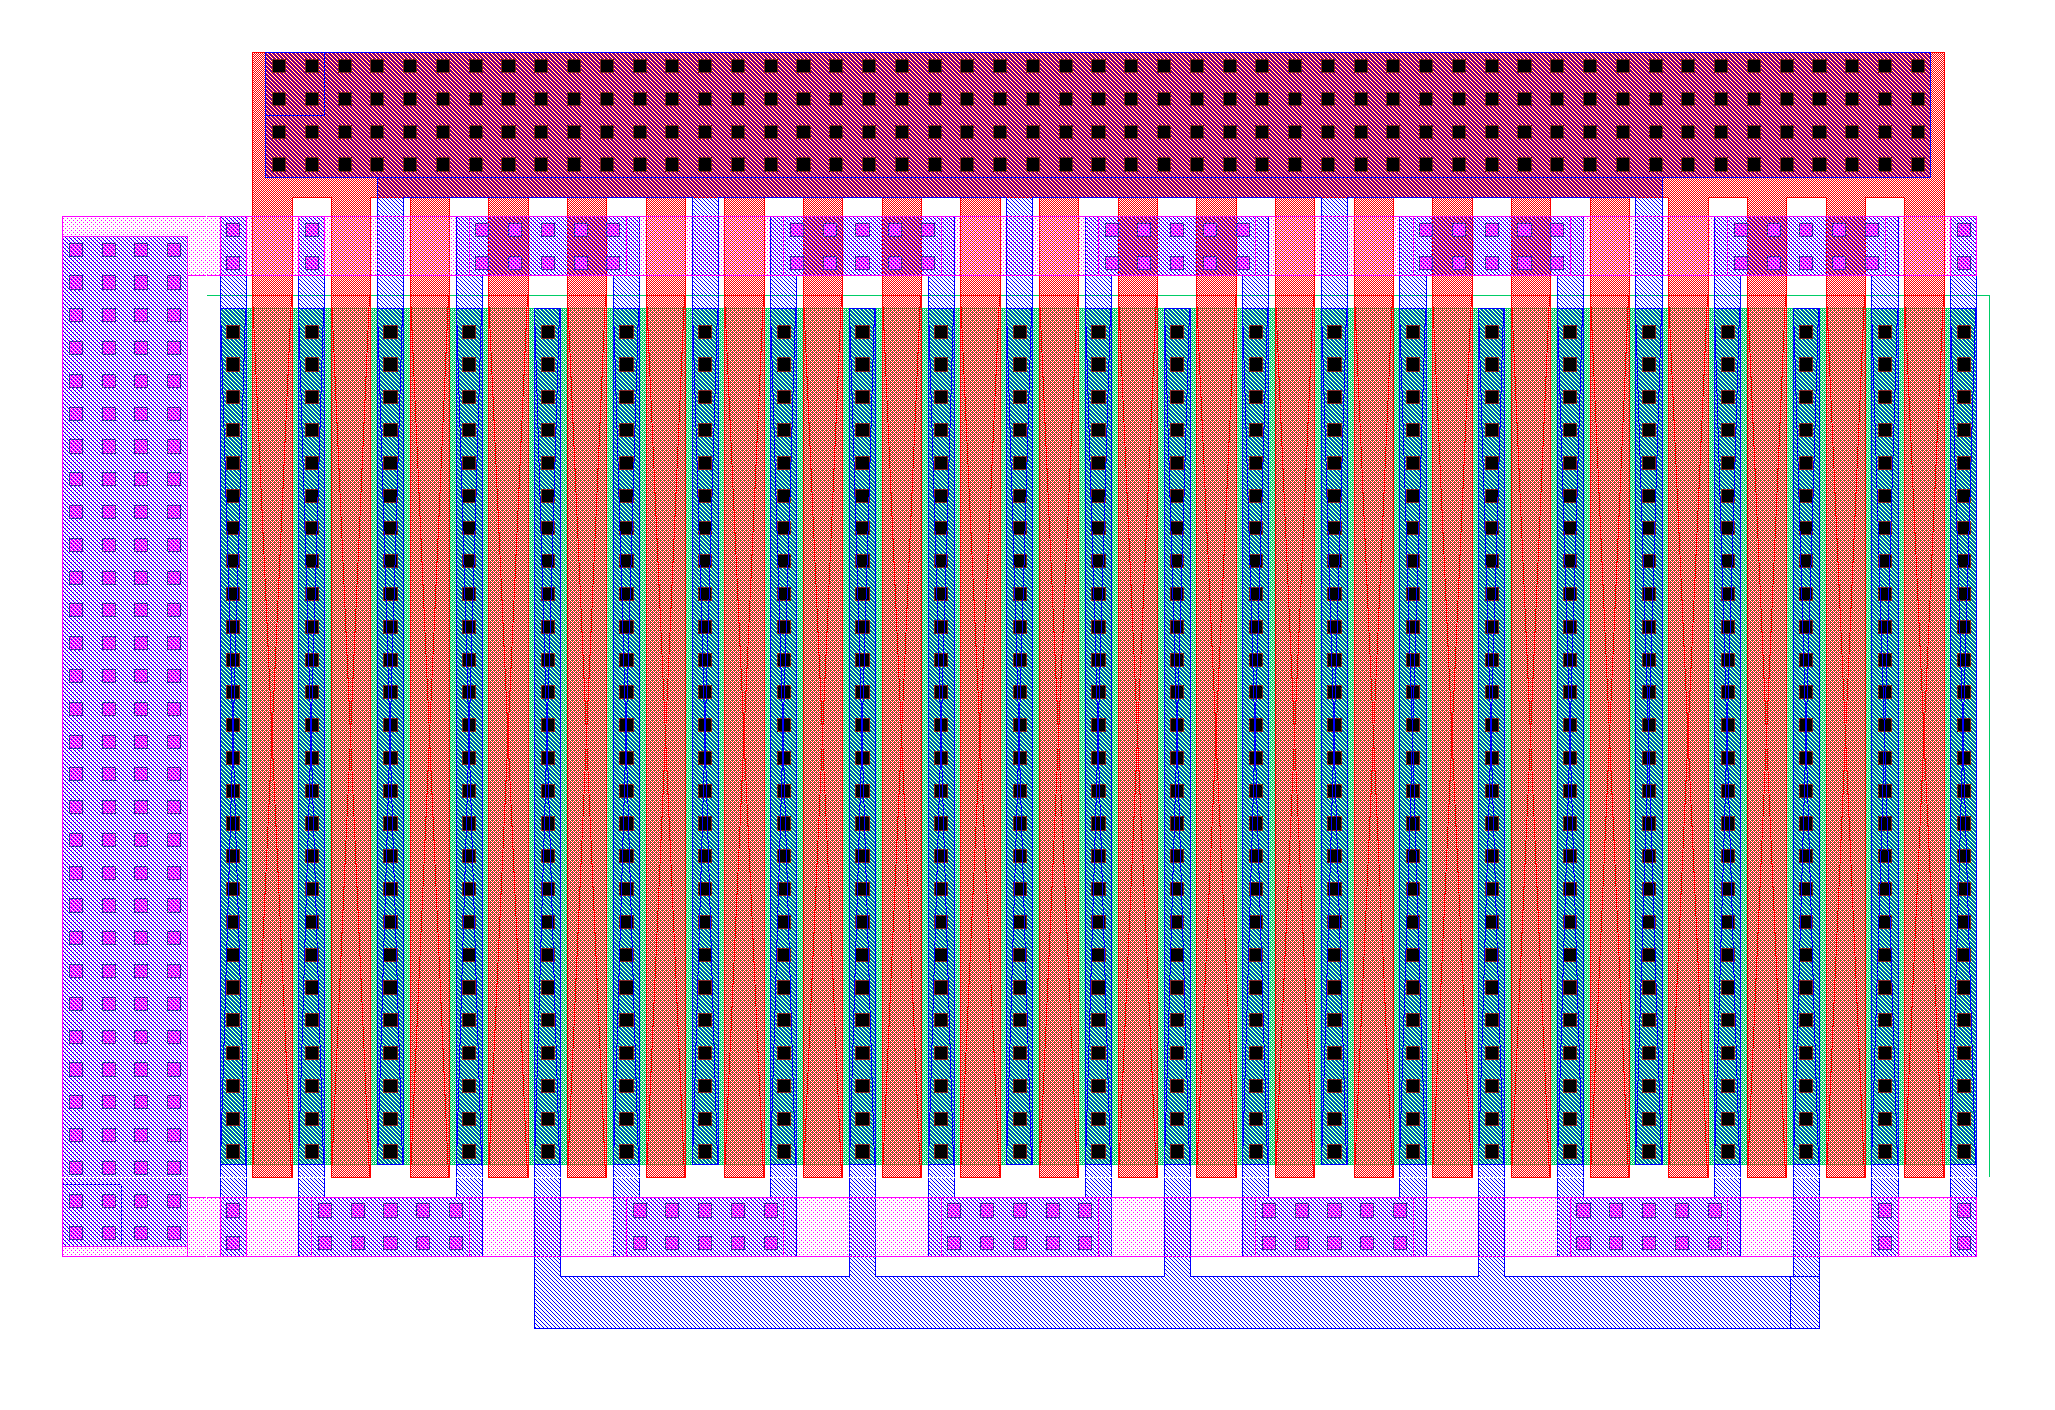
\includegraphics[width=\textwidth]{L_curmir_full}
	\caption{Complete layout of current mirror}
	\label{L_curmir_full}
\end{figure}

Concerning the diode-connected transistor M5, interdigitated structure was implemented. Dummy transistors are placed aside whereas an array of contacts to minimize series resistance between gate and drain has been added. Final layouts and highlighted nets are visible in figure \ref{L_M5_full}. 
\begin{figure}[H]
	\centering
	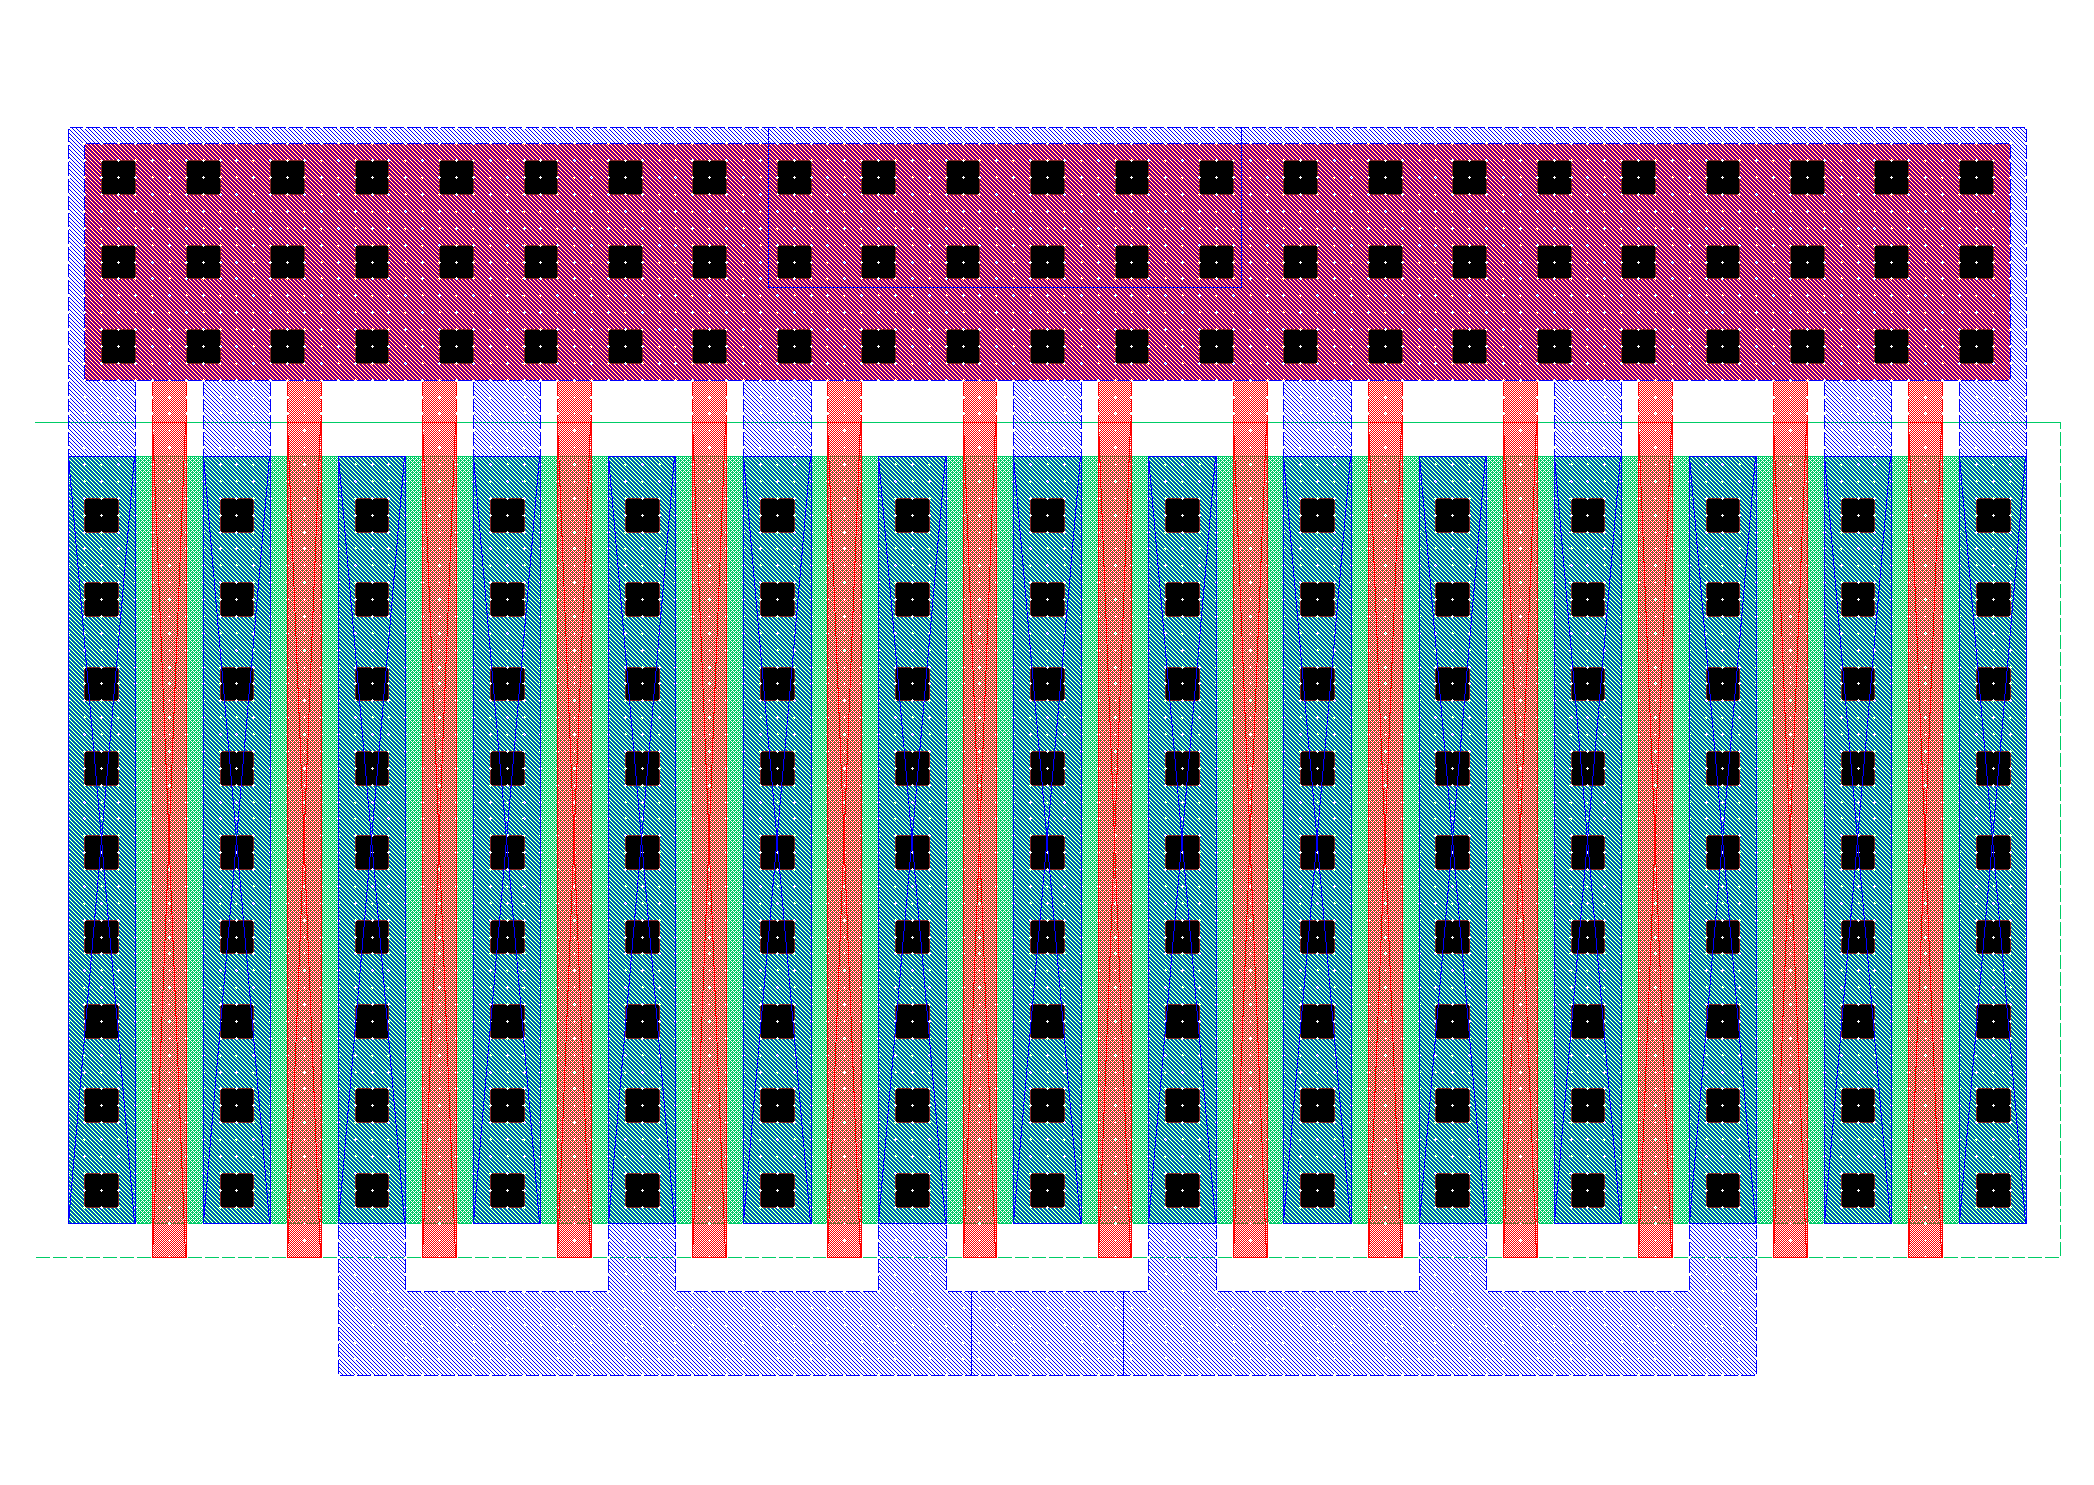
\includegraphics[width=0.75\textwidth]{L_M5_full}
	\caption{Complete layout of M5 transistor}
	\label{L_M5_full}
\end{figure}

\subsection{Capacitors}
\paragraph{Bias capacitors}
Bias capacitors have been designed using two configurations of common centroid layout.
A simplified version of the layout structure implemented is drawn in figure \ref{Cap1}. 
\begin{figure}[H]
	\centering
	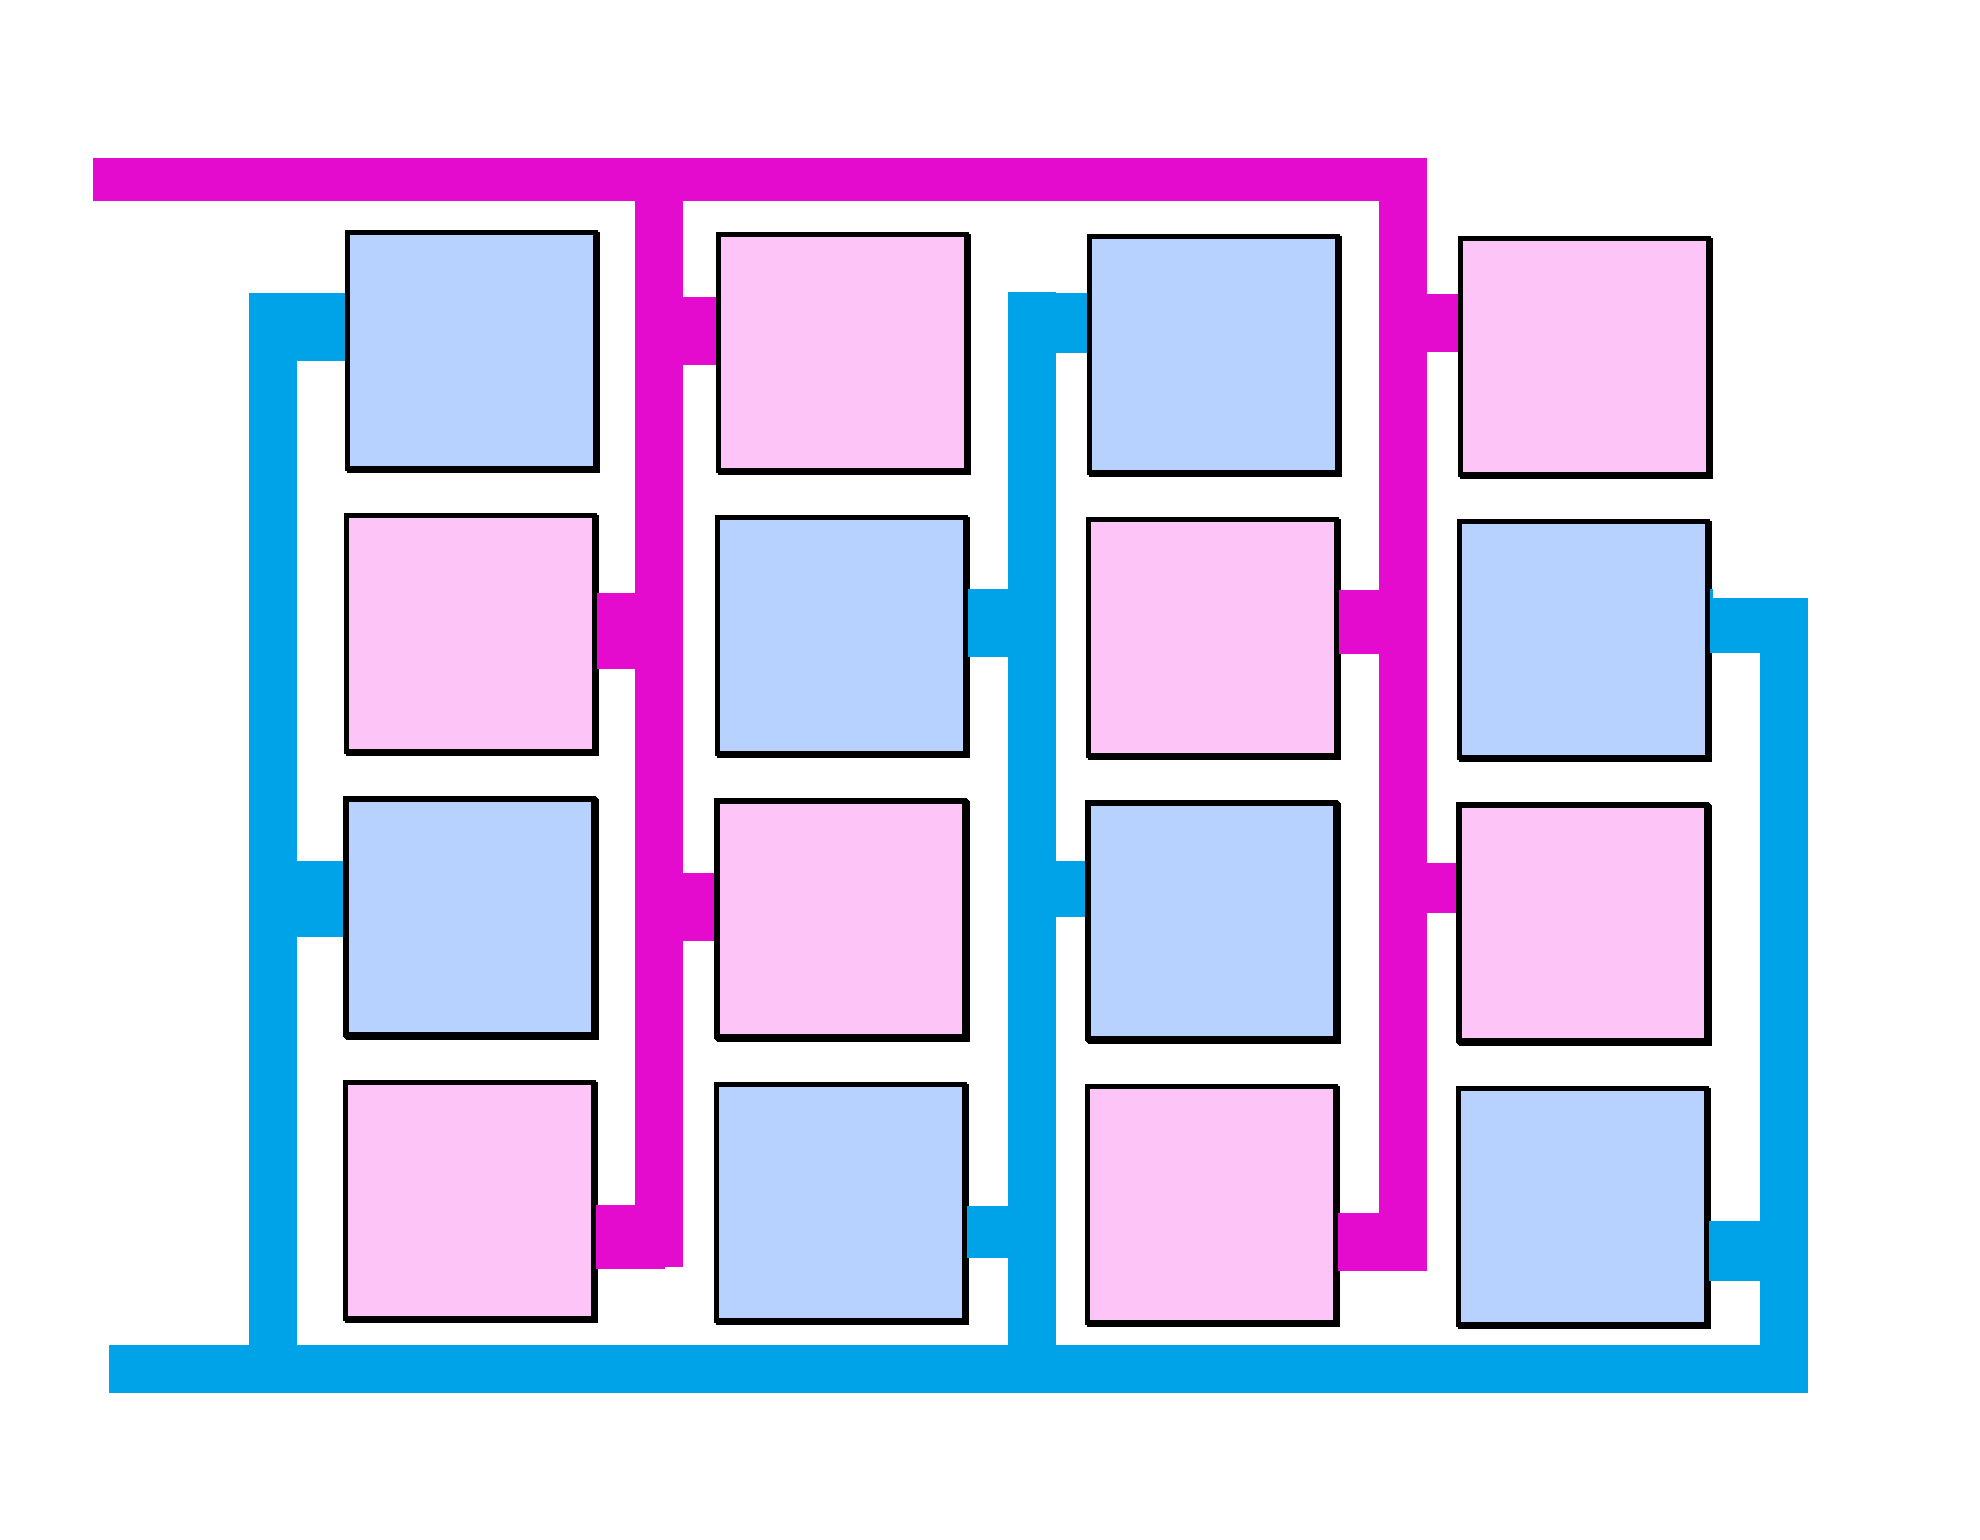
\includegraphics[width=0.6\textwidth]{Cap1}
	\caption{Bias capacitors layout structure}
	\label{Cap1}
\end{figure}
Even if no exact ratio between the two capacitors is needed, a modular geometry, made by equal squares, was used. This minimizes undercut effects, and the square shape reduces border errors. In order to reduce the area, capacitor units were designed using poly1 and poly2 (elec) layers, which give the maximum capacitance per unit area available with this technology kit. A dummy capacitor frame was placed around to minimize border effect. All the capacitors lie above an n-well, whose purpose is to minimize fringing field leakage. This n-well is tied to \(V_{DD}\) potential. The final layout with highlighted nets is visible in figure \ref{L_Cb_full}.
\begin{figure}[H]
	\centering
	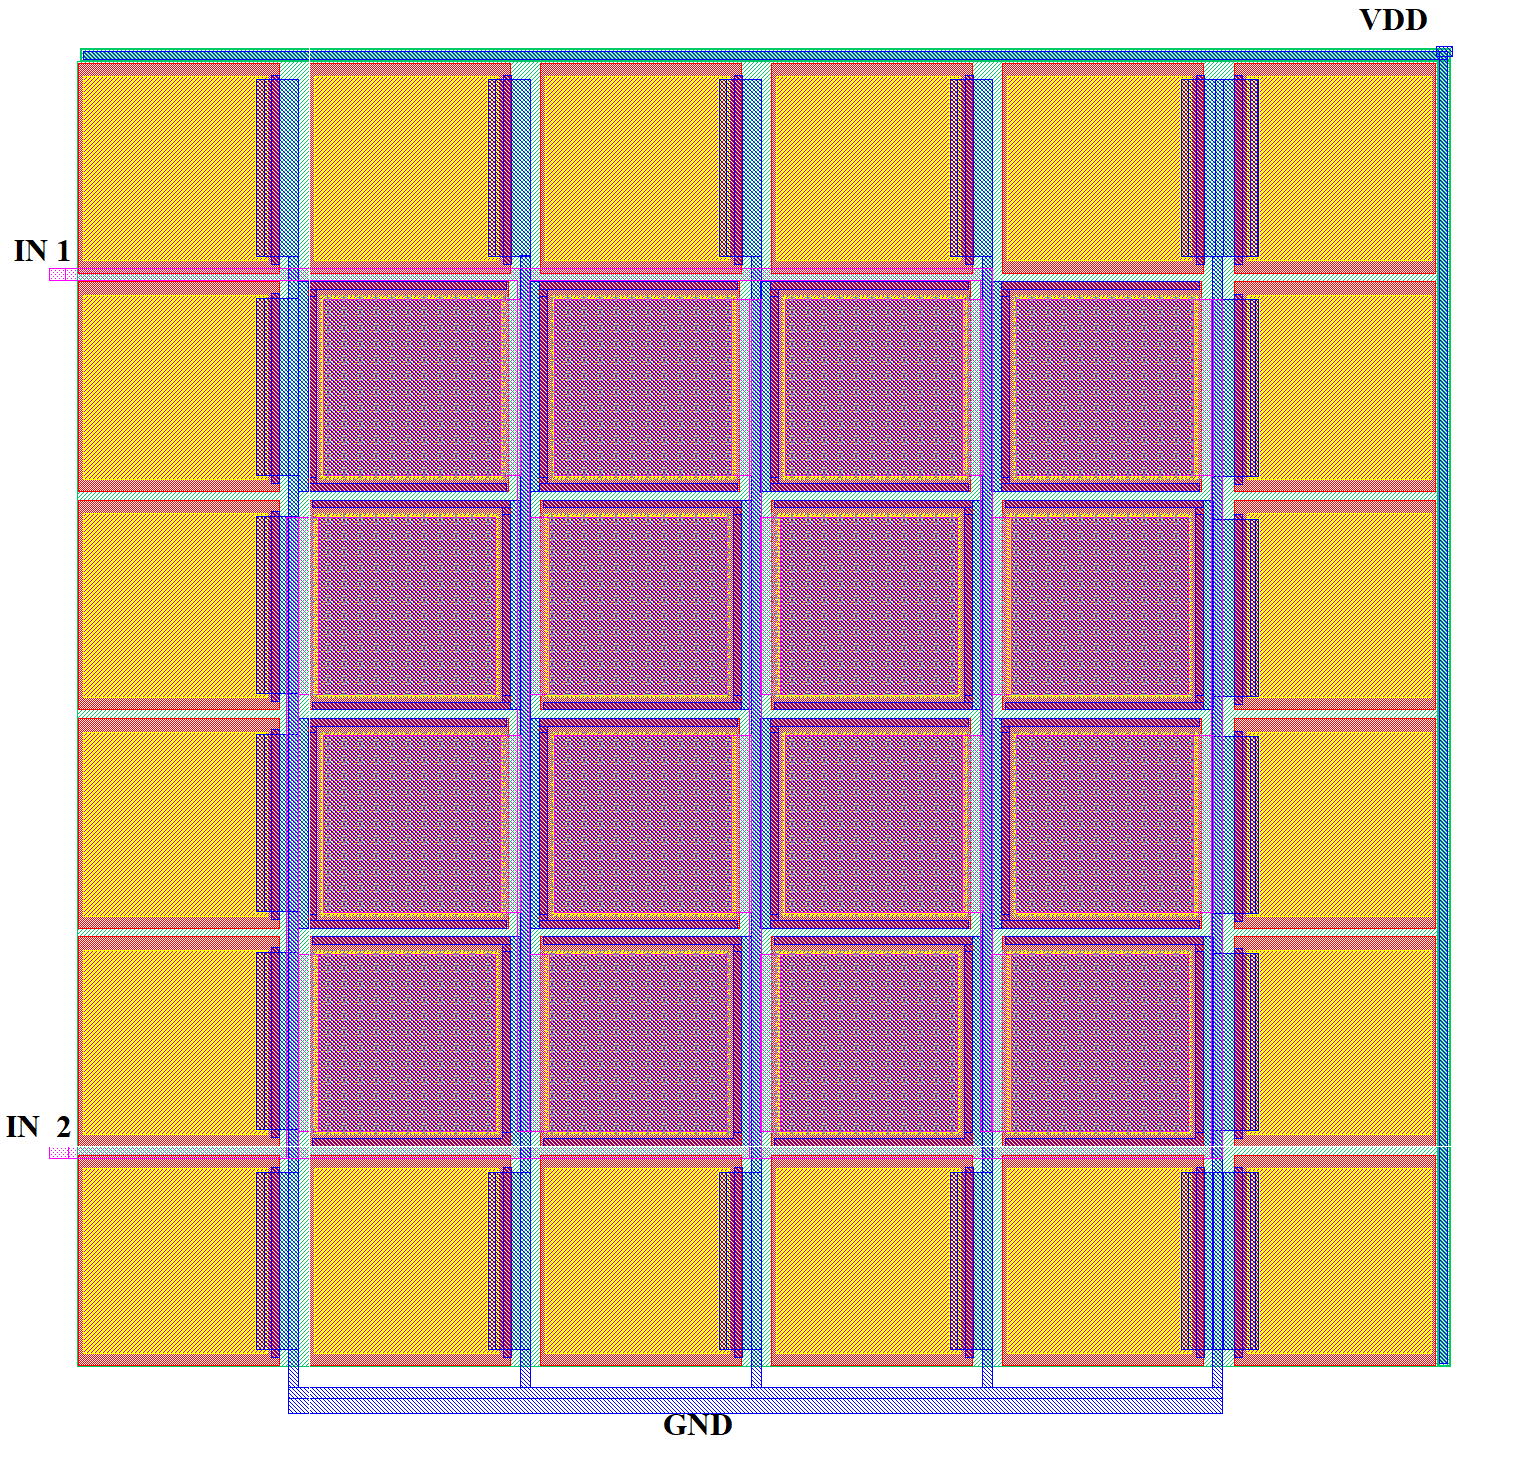
\includegraphics[width=0.6\textwidth]{L_Cb_full}
	\caption{Full layout of \(C_{bias}\) capacitors}
	\label{L_Cb_full}
\end{figure}

\paragraph{Signal capacitors}
Since these capacitors resulted to be very space demanding due to capacitance value, a multi-layer capacitor was tried to be built alternating poly and metal layers. Unfortunately this idea was soon abandoned due to the \emph{rule 11.6 of SCMOS} rules, which does not allow unrelated metal layer over poly2. The most practical solution proven to be using poly1-to-poly2 capacitance in a common centroid structure. This time matching is more important with respect to bias capacitors, because we want signal coming to the differential stages pass through strongly symmetrical paths.
A simplified version of the common centroid structure implemented is shown in figure \ref{Cap2}. 
\begin{figure}[H]
	\centering
	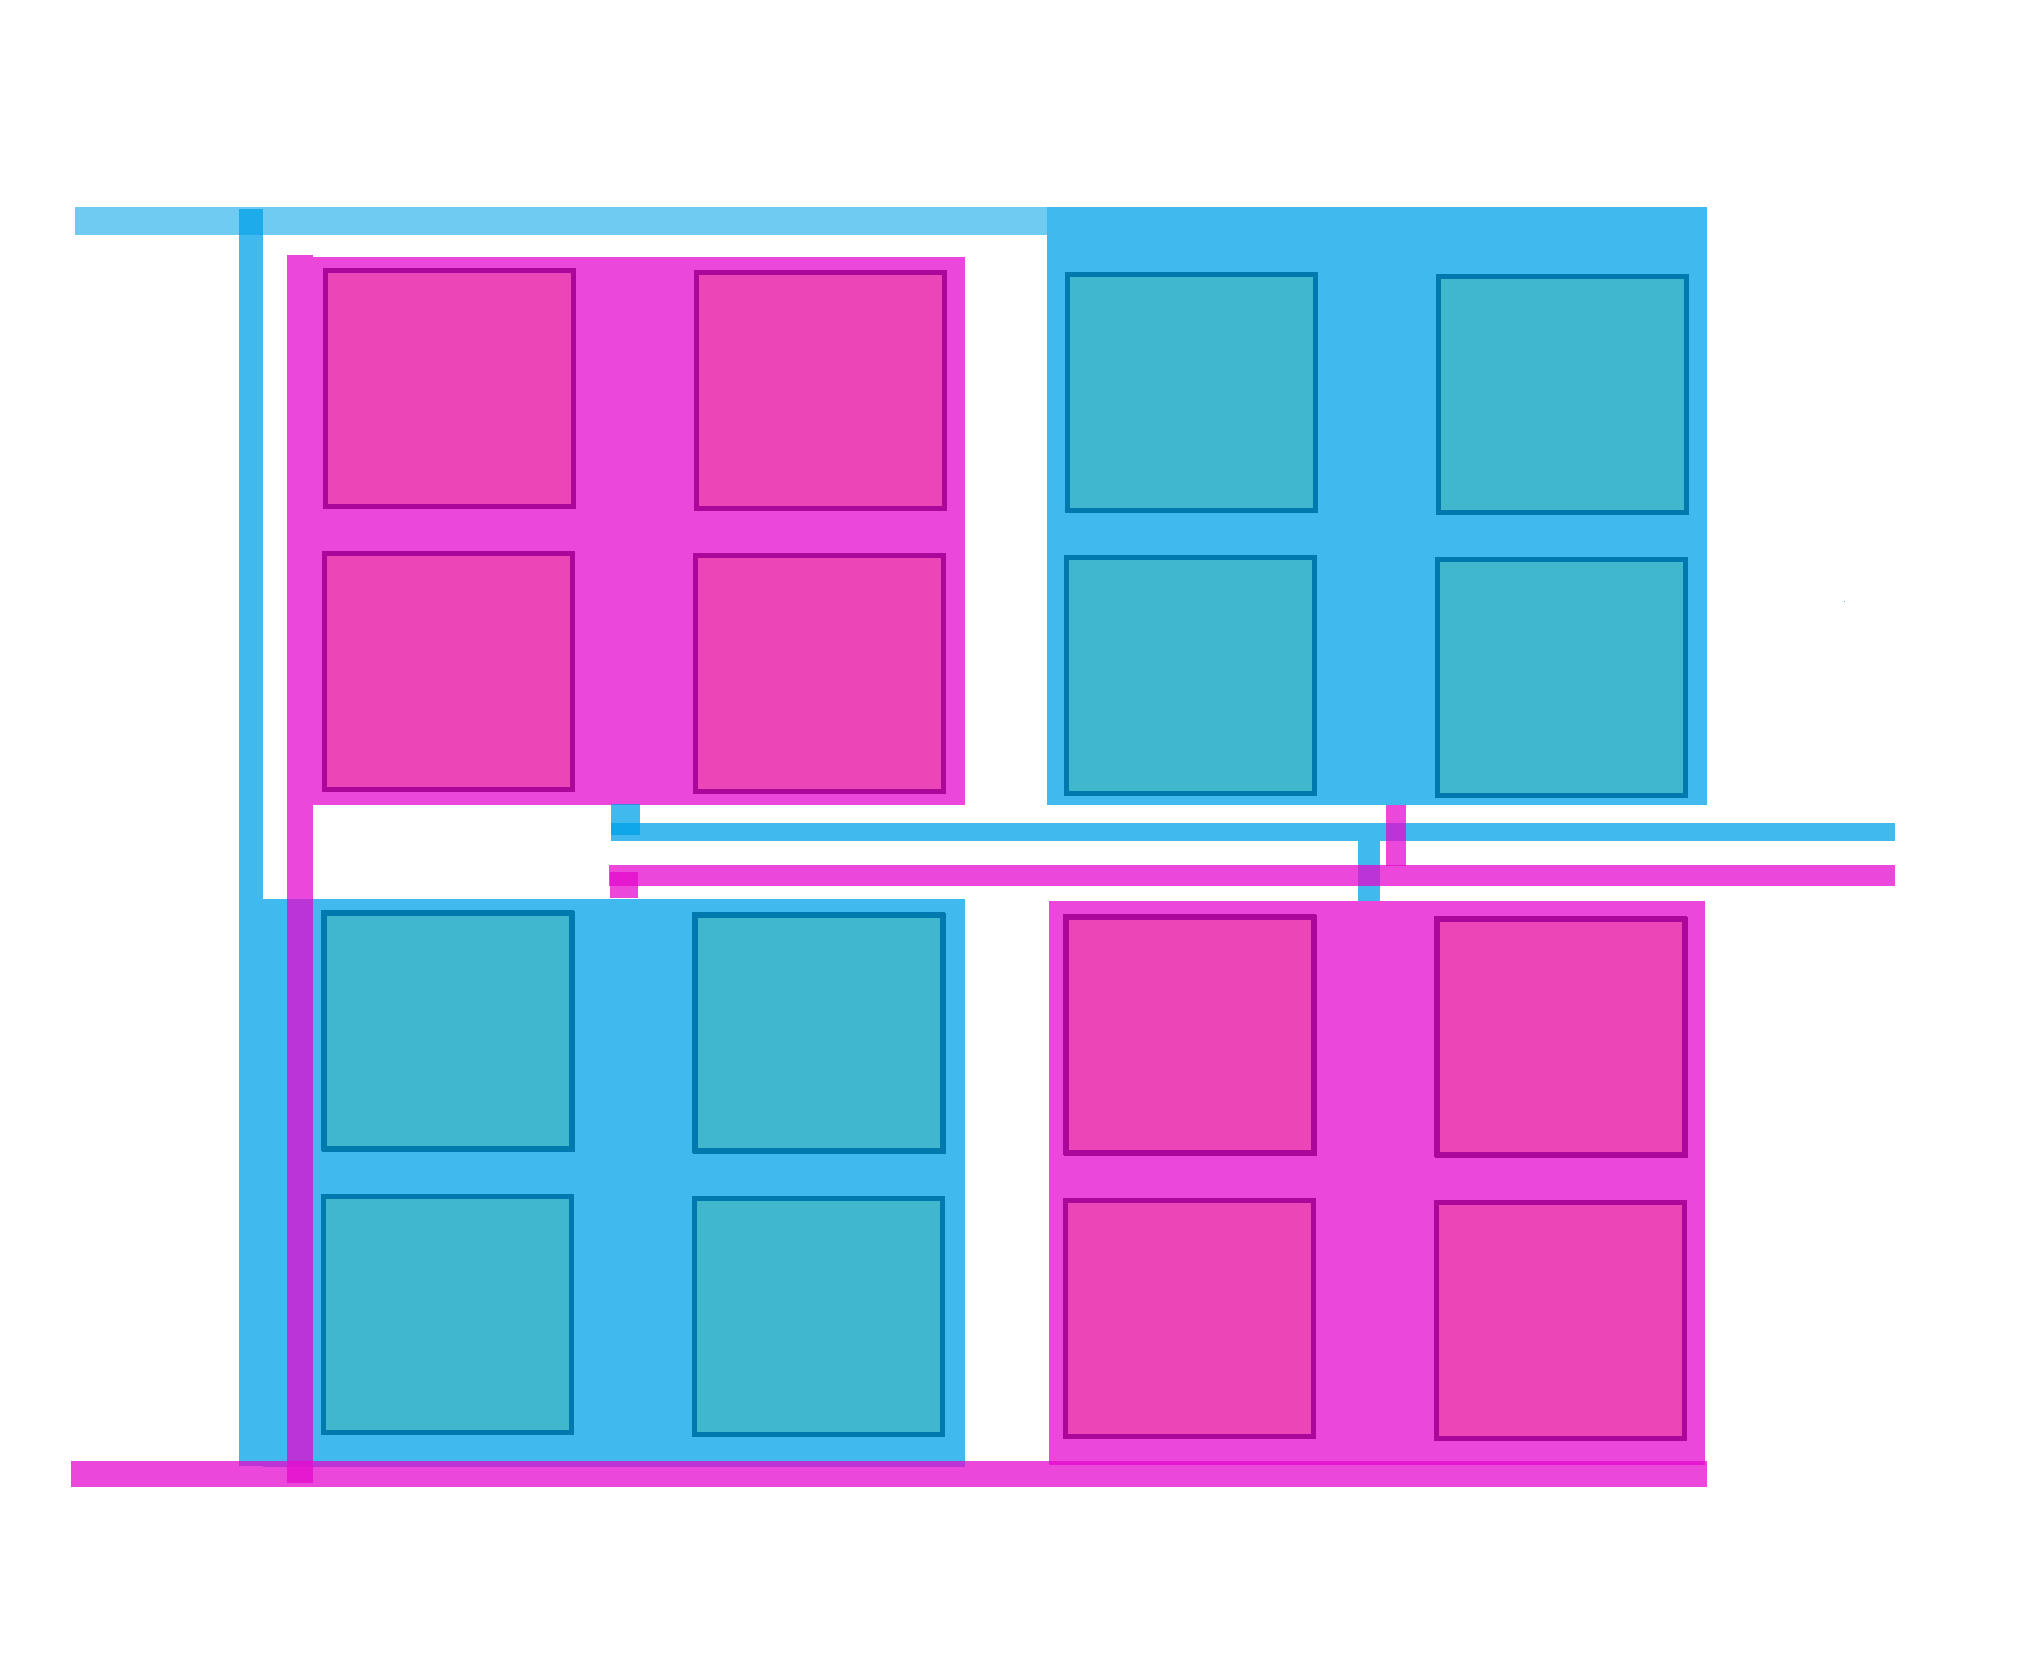
\includegraphics[width=0.6\textwidth]{Cap2}
	\caption{Common centroid structure of the signal capacitors}
	\label{Cap2}
\end{figure}
Since this is a high frequency path to reduce series resistance and inductance, metal plates with contacts were placed all over the square unit capacitors. Dummy short circuited elements were positioned all around the capacitor as well. An additional n-well connected to \(V_{DD}\) surrounds the capacitor to reduce fringing field leakage. The overall capacitance layout with highlighted nets is visible in figure \ref{L_Cs_full}.
\begin{figure}[H]
	\centering
	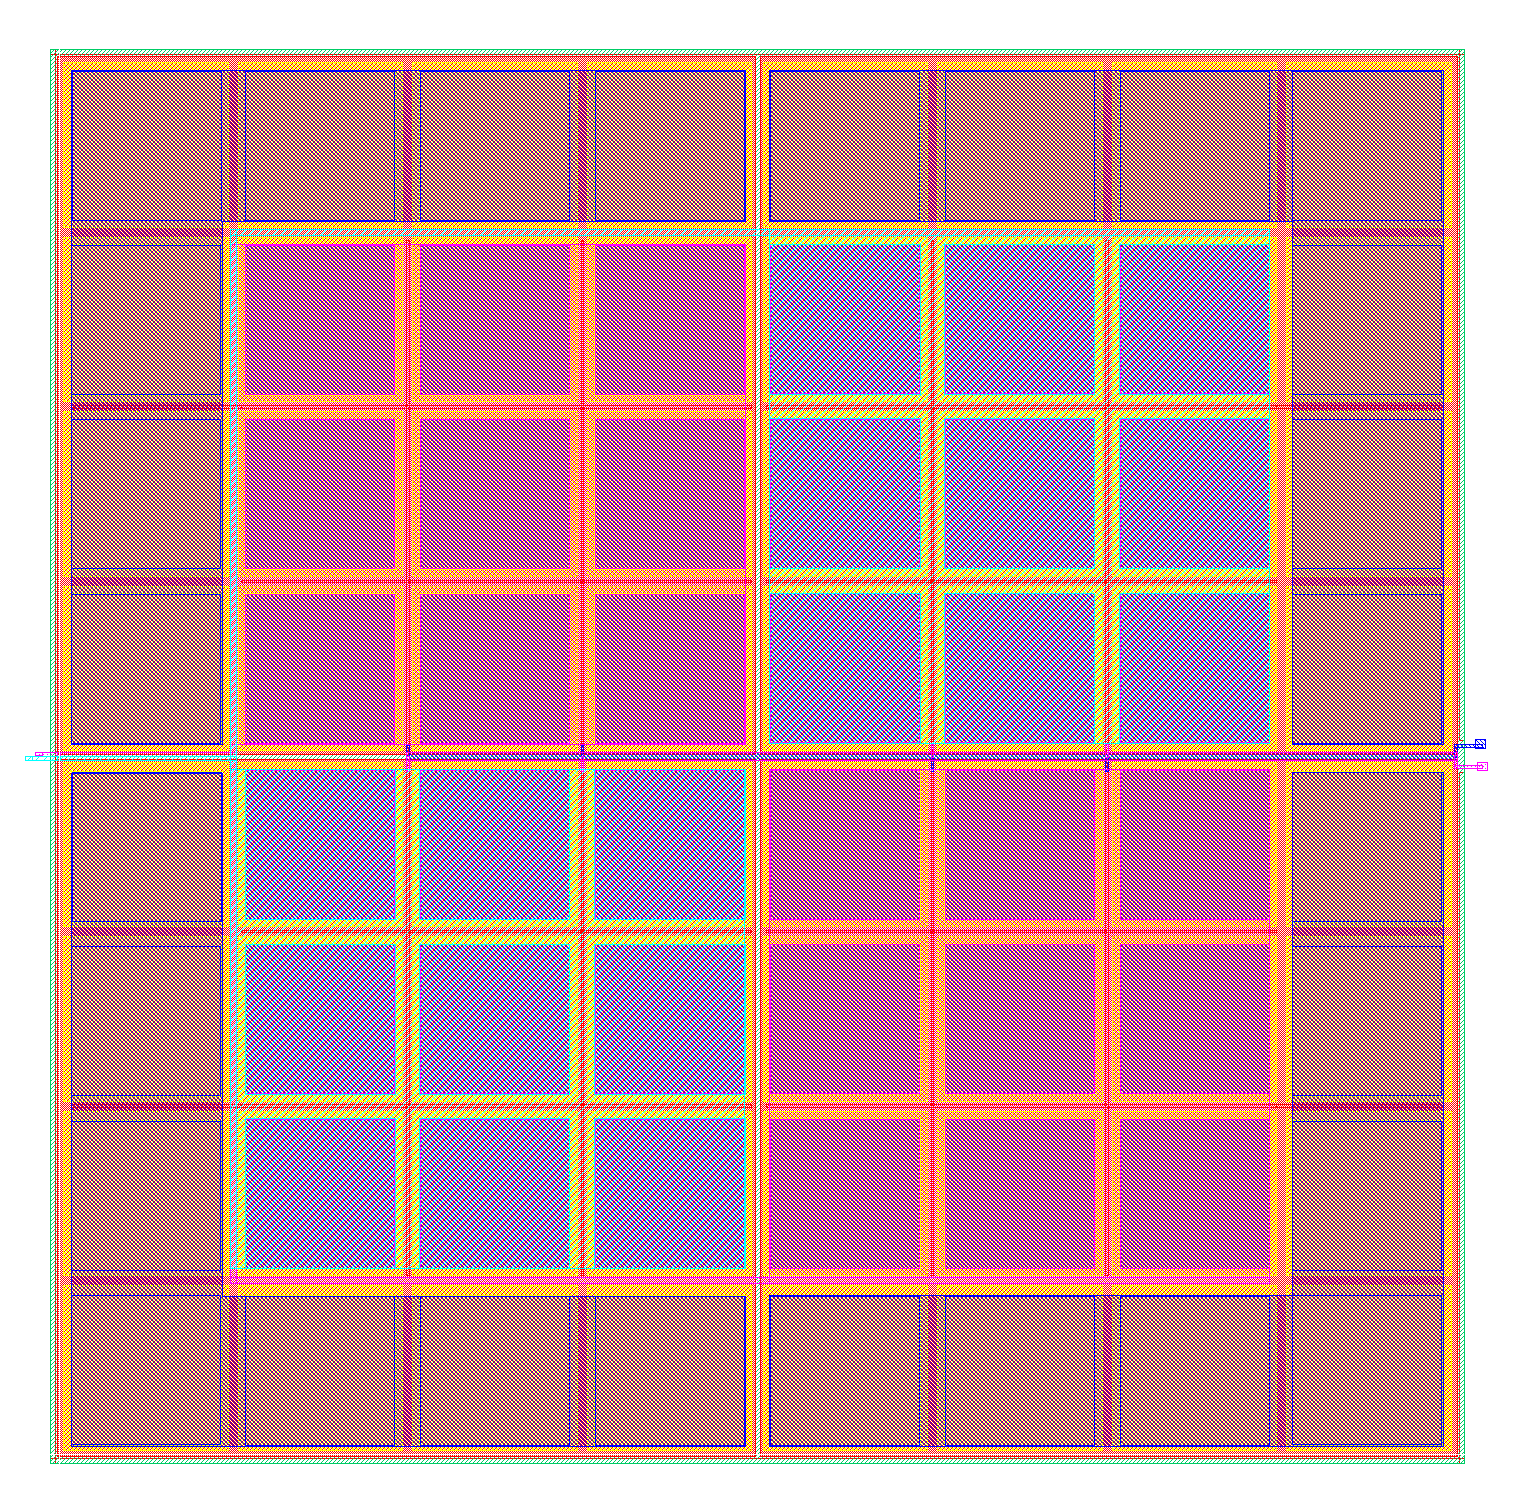
\includegraphics[width=0.7\textwidth]{L_Cs_full}
	\caption{Full layout of \(C_{signal}\) capacitors}
	\label{L_Cs_full}
\end{figure}

\subsection{Resistors}
Two kinds of resistors have been implemented in this layout, both of them are described in the following paragraphs.
\paragraph{N-well resistors}
Resistors fabricated in n-well have worse tolerance, but an higher sheet resistance. That's the way this kind of resistor was chosen to implement biasing resistors \(R_1\) and \(R_3\), which are, as a matter of fact, very large in absolute value, but their tolerance is not too important. We can thus have smaller layout adopting n-well layout. Resistors were split in modular structures with the common centroid fashion to reduce differences between \(R_1\) and \(R_3\). Due to the fact that this resistors are very close to the mixing stage, a guard ring connected to ground has been included to prevent substrate noise being injected through the biasing network. The final layout obtained for \(R_1\) and \(R_3\) resistor is visible in \ref{L_R1R3}.
 
\begin{figure}[H]
	\centering
	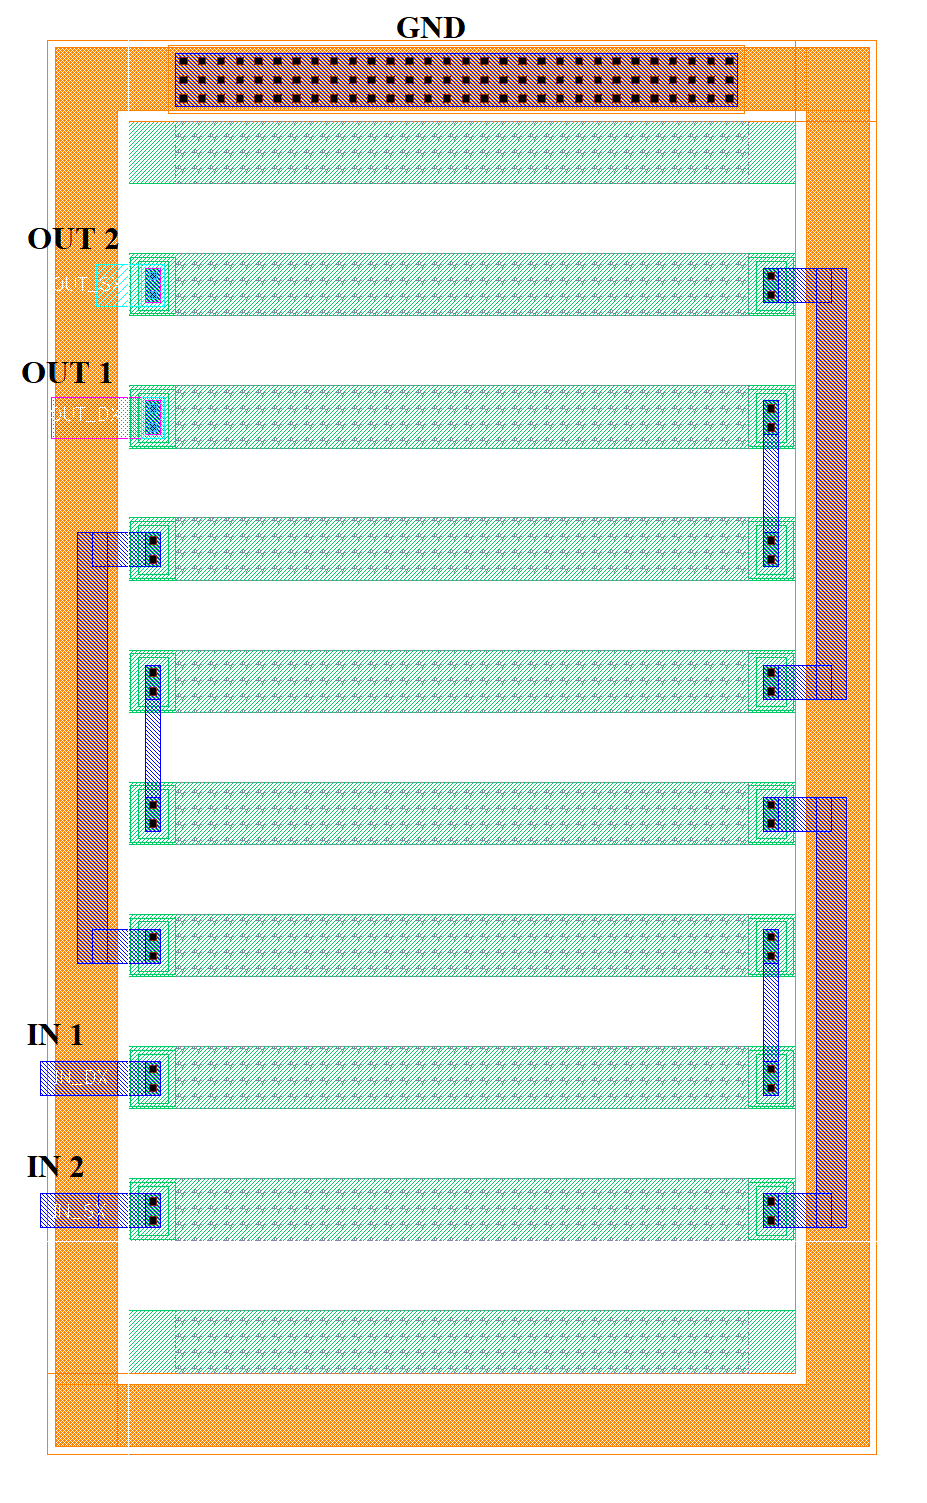
\includegraphics[scale=0.2]{L_R1R3}
	\caption{Layout of $R_1$ and $R_3$ resistors}
	\label{L_R1R3}
\end{figure}

\paragraph{Poly silicon resistors}
Since other resistors are smaller than \(R_1\) and \(R_3\), poly has been employed to build them, taking advantage of their higher precision but smaller sheet resistance. All of them were drawn in common centroid structure, except for \(R_4\) (due to its small value), and dummy elements on both sides were always used. Final layouts for these resistors are shown in \ref{subfig-1:L_R2},\ref{subfig-1:L_R4},\ref{subfig-1:L_RL},\ref{subfig-1:L_RS}. Dimensions are not in scale.

\begin{figure}[H]
	\centering
	
	\subfloat[$R_2$\label{subfig-1:L_R2}]
	{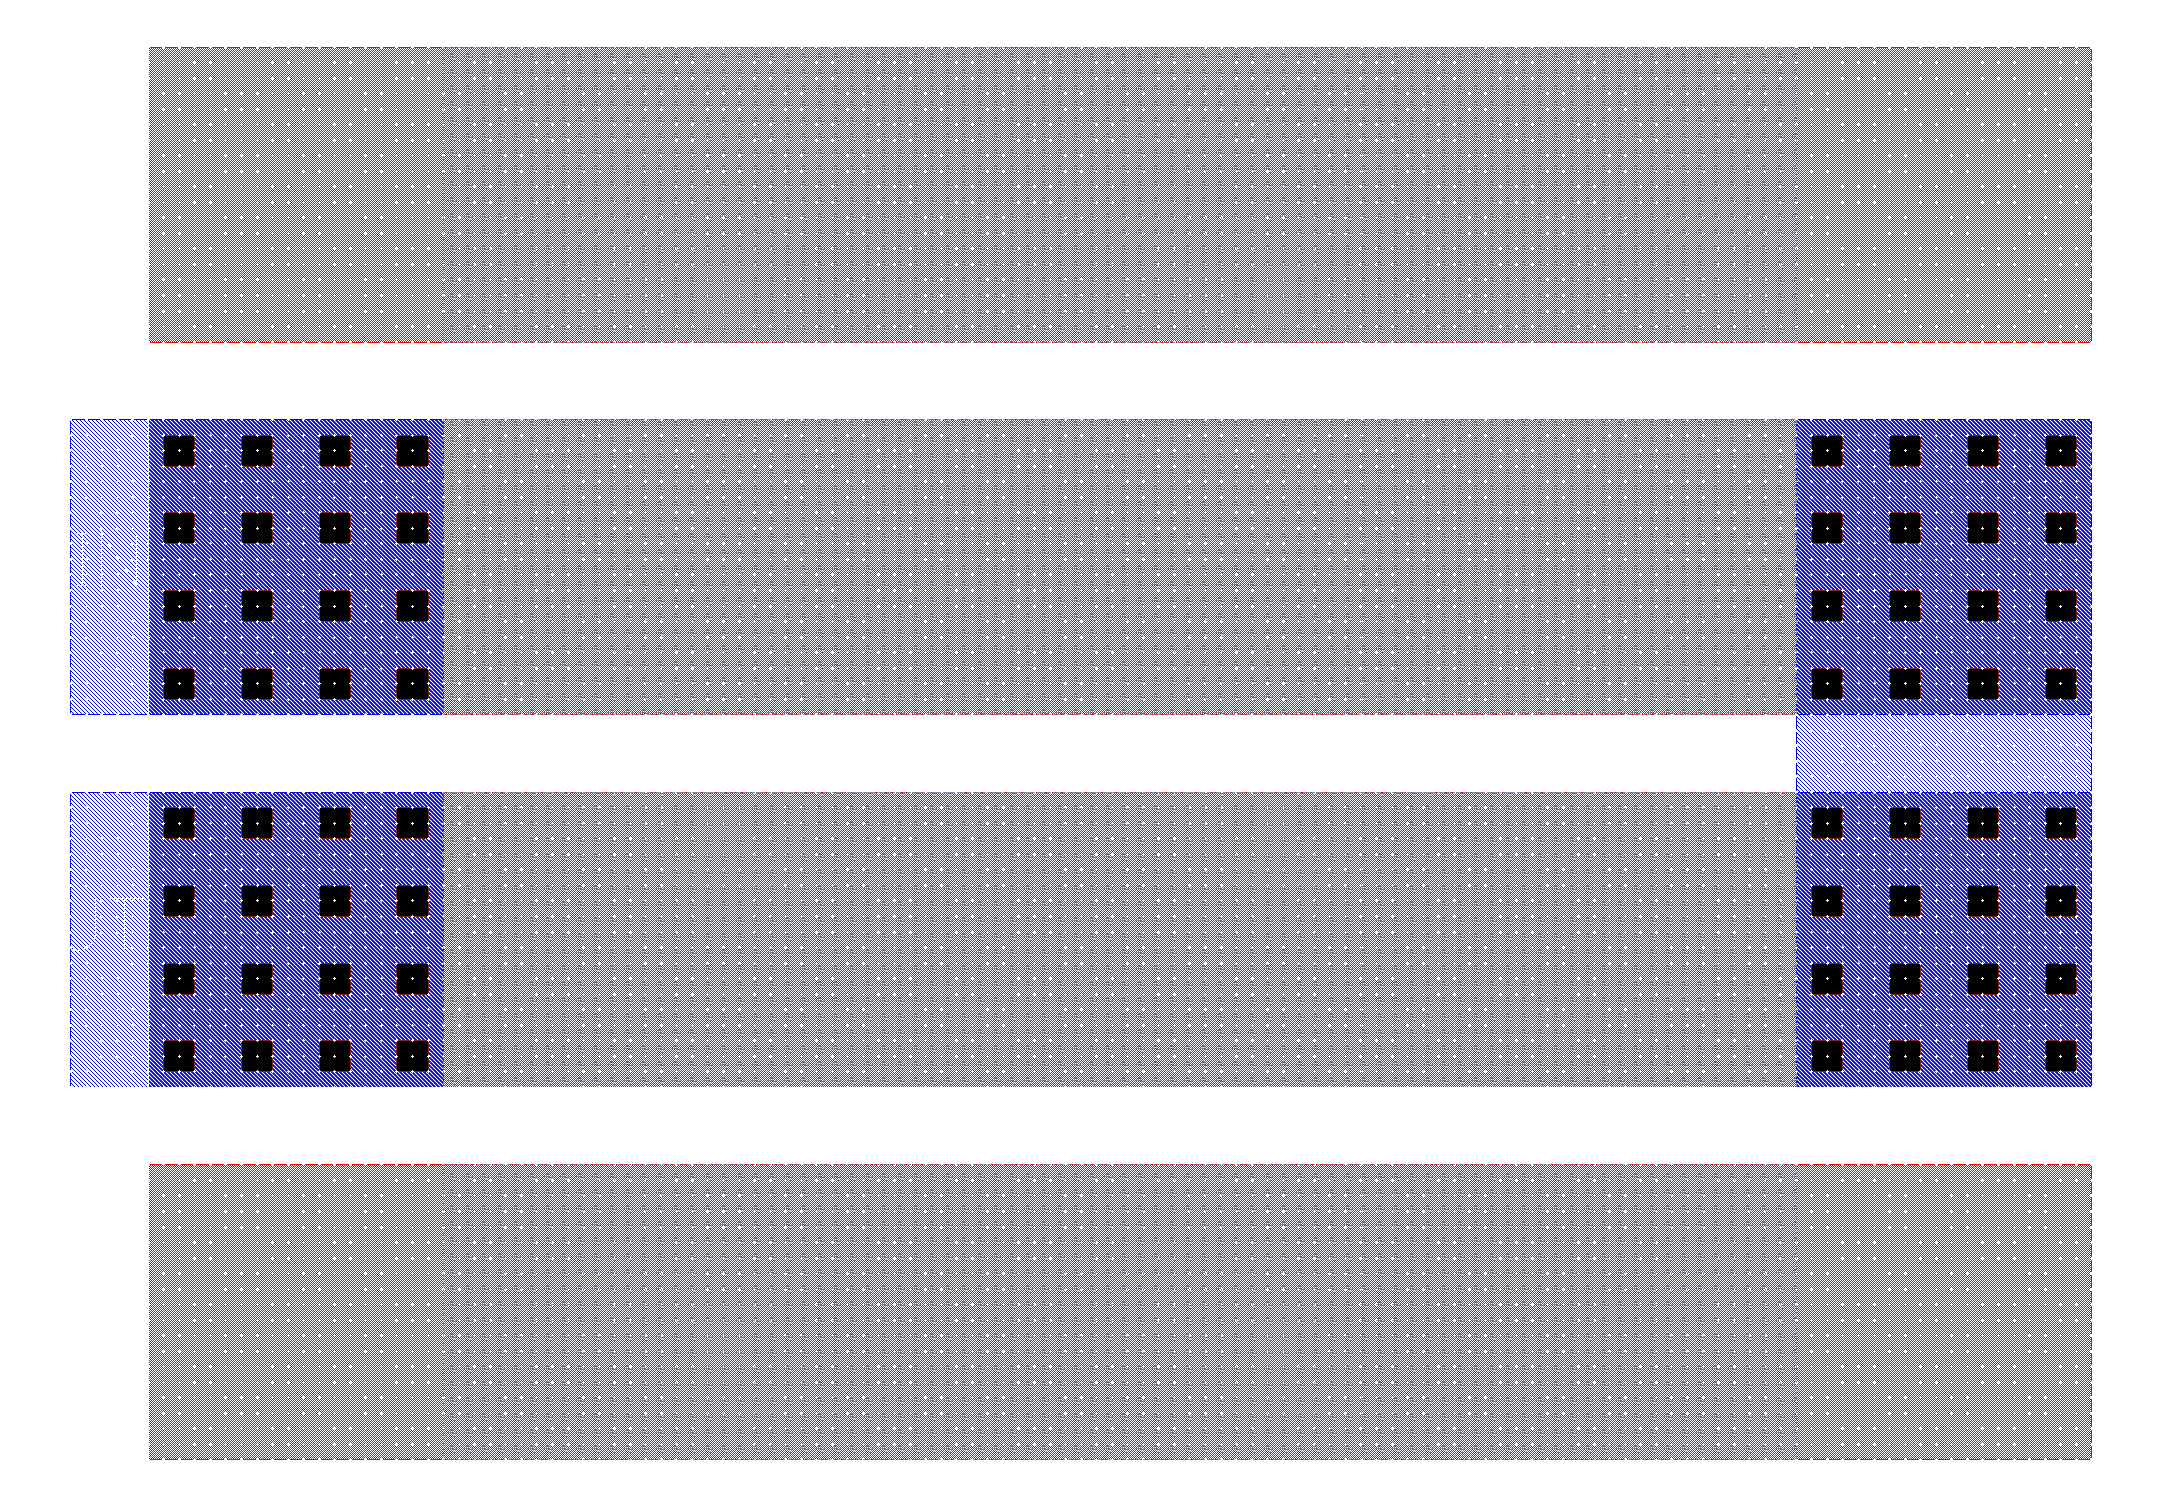
\includegraphics[width=0.4\textwidth]{L_R2}}
	\subfloat[$R_4$\label{subfig-1:L_R4}]
	{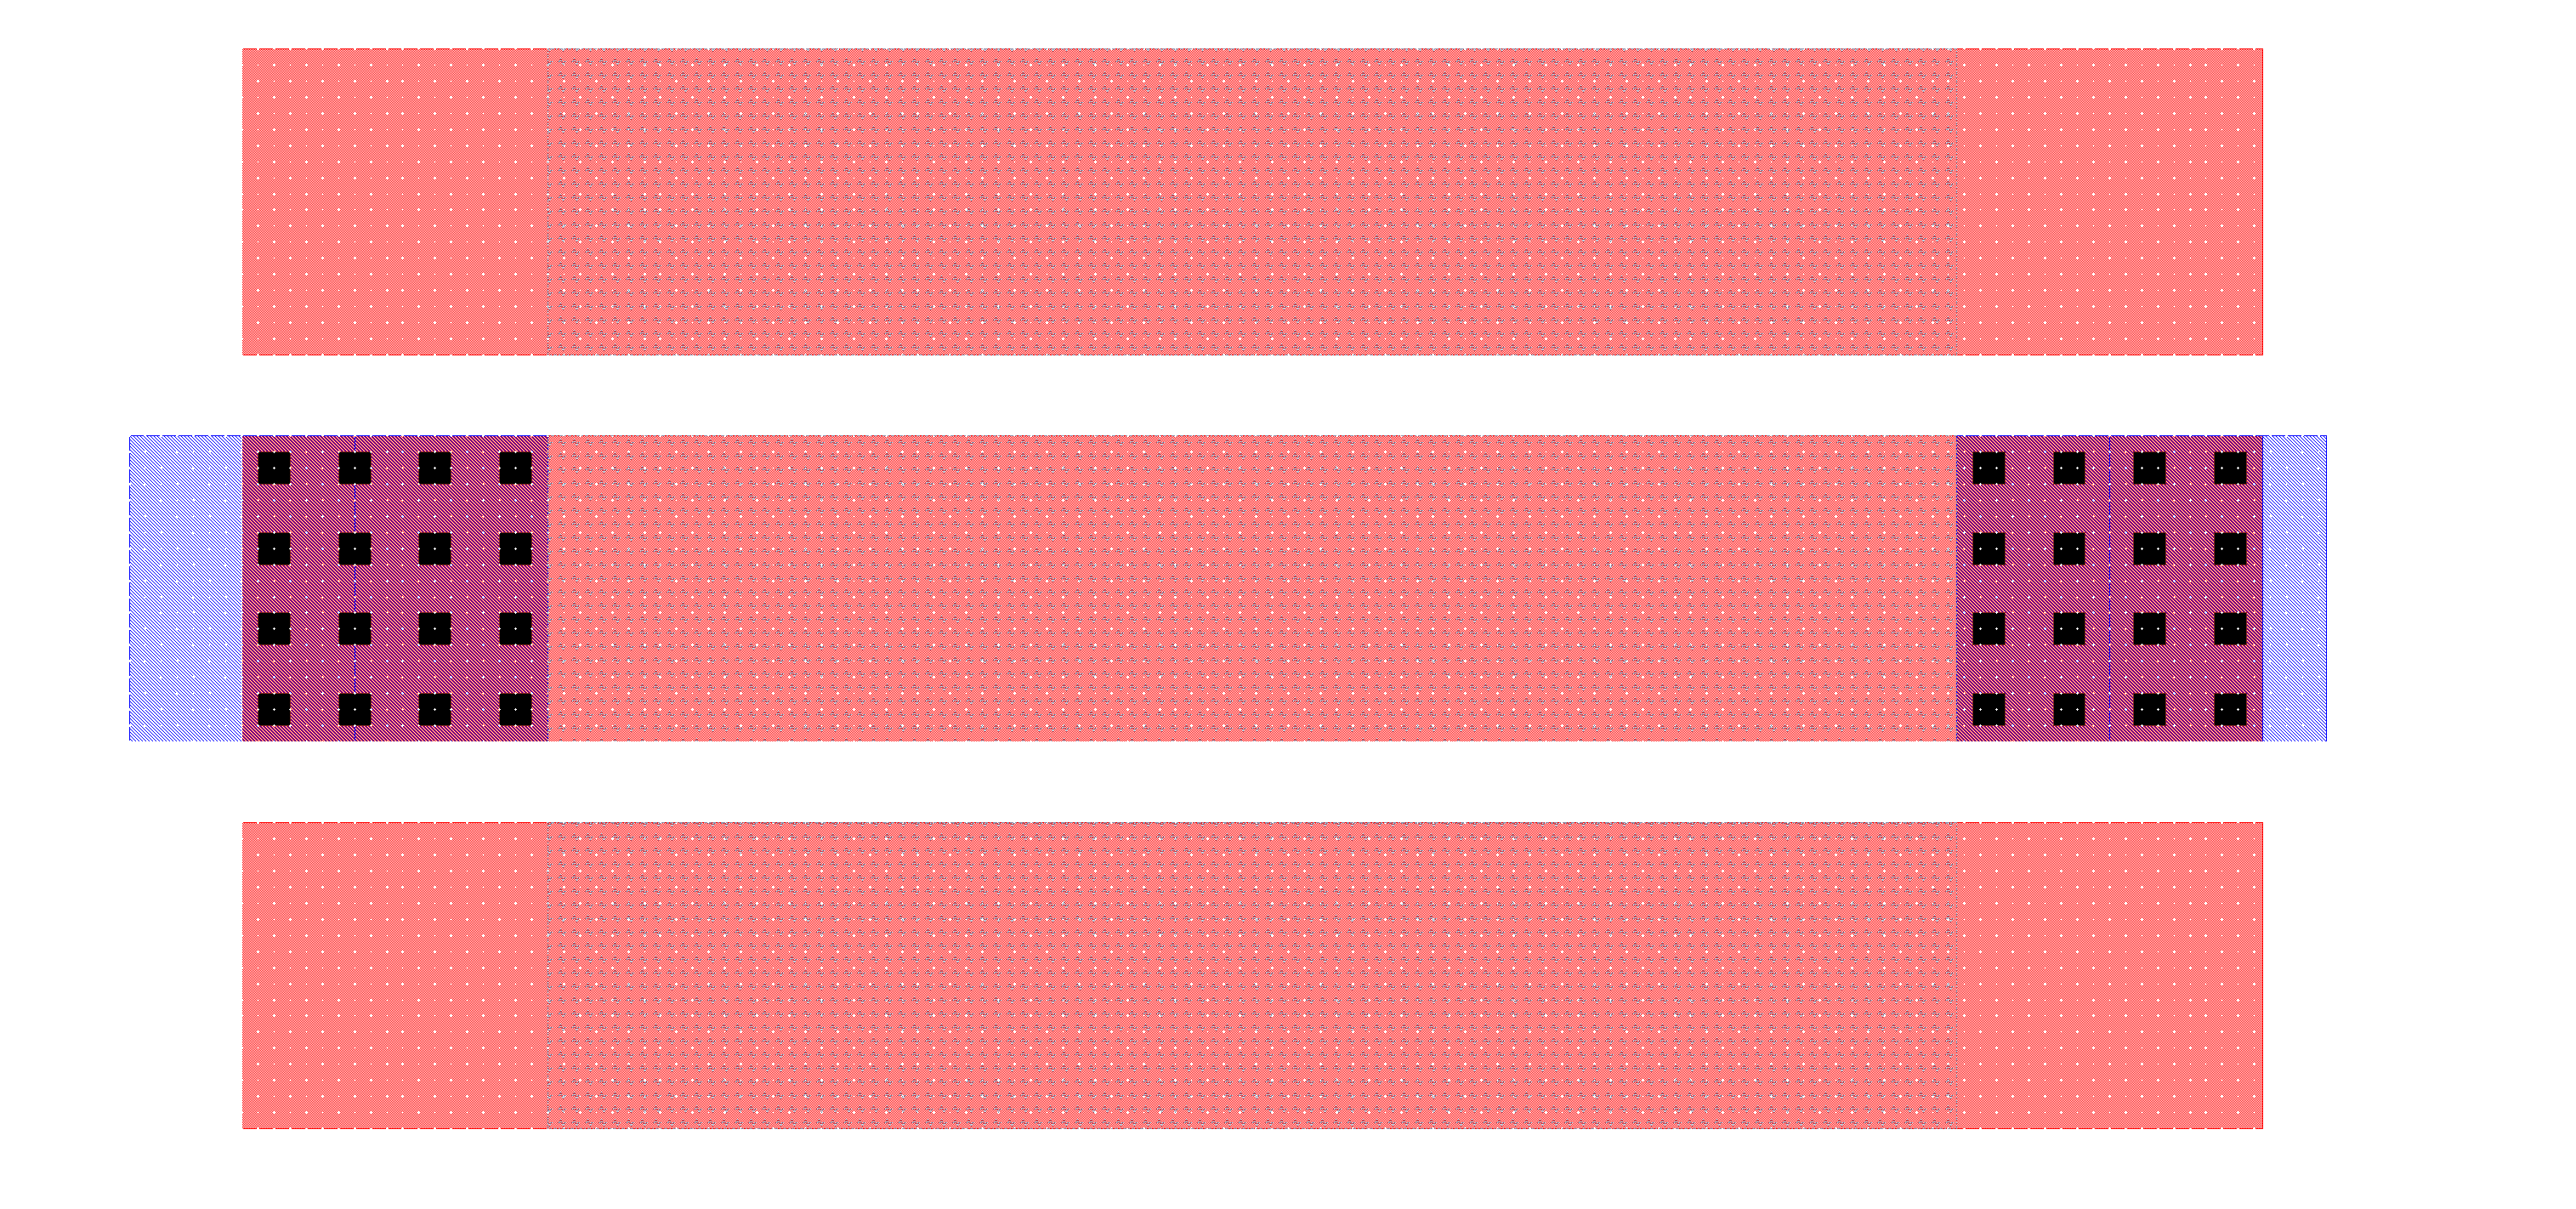
\includegraphics[width=0.5\textwidth]{L_R4}}
	\vfill
	\subfloat[$R_L$\label{subfig-1:L_RL}]
	{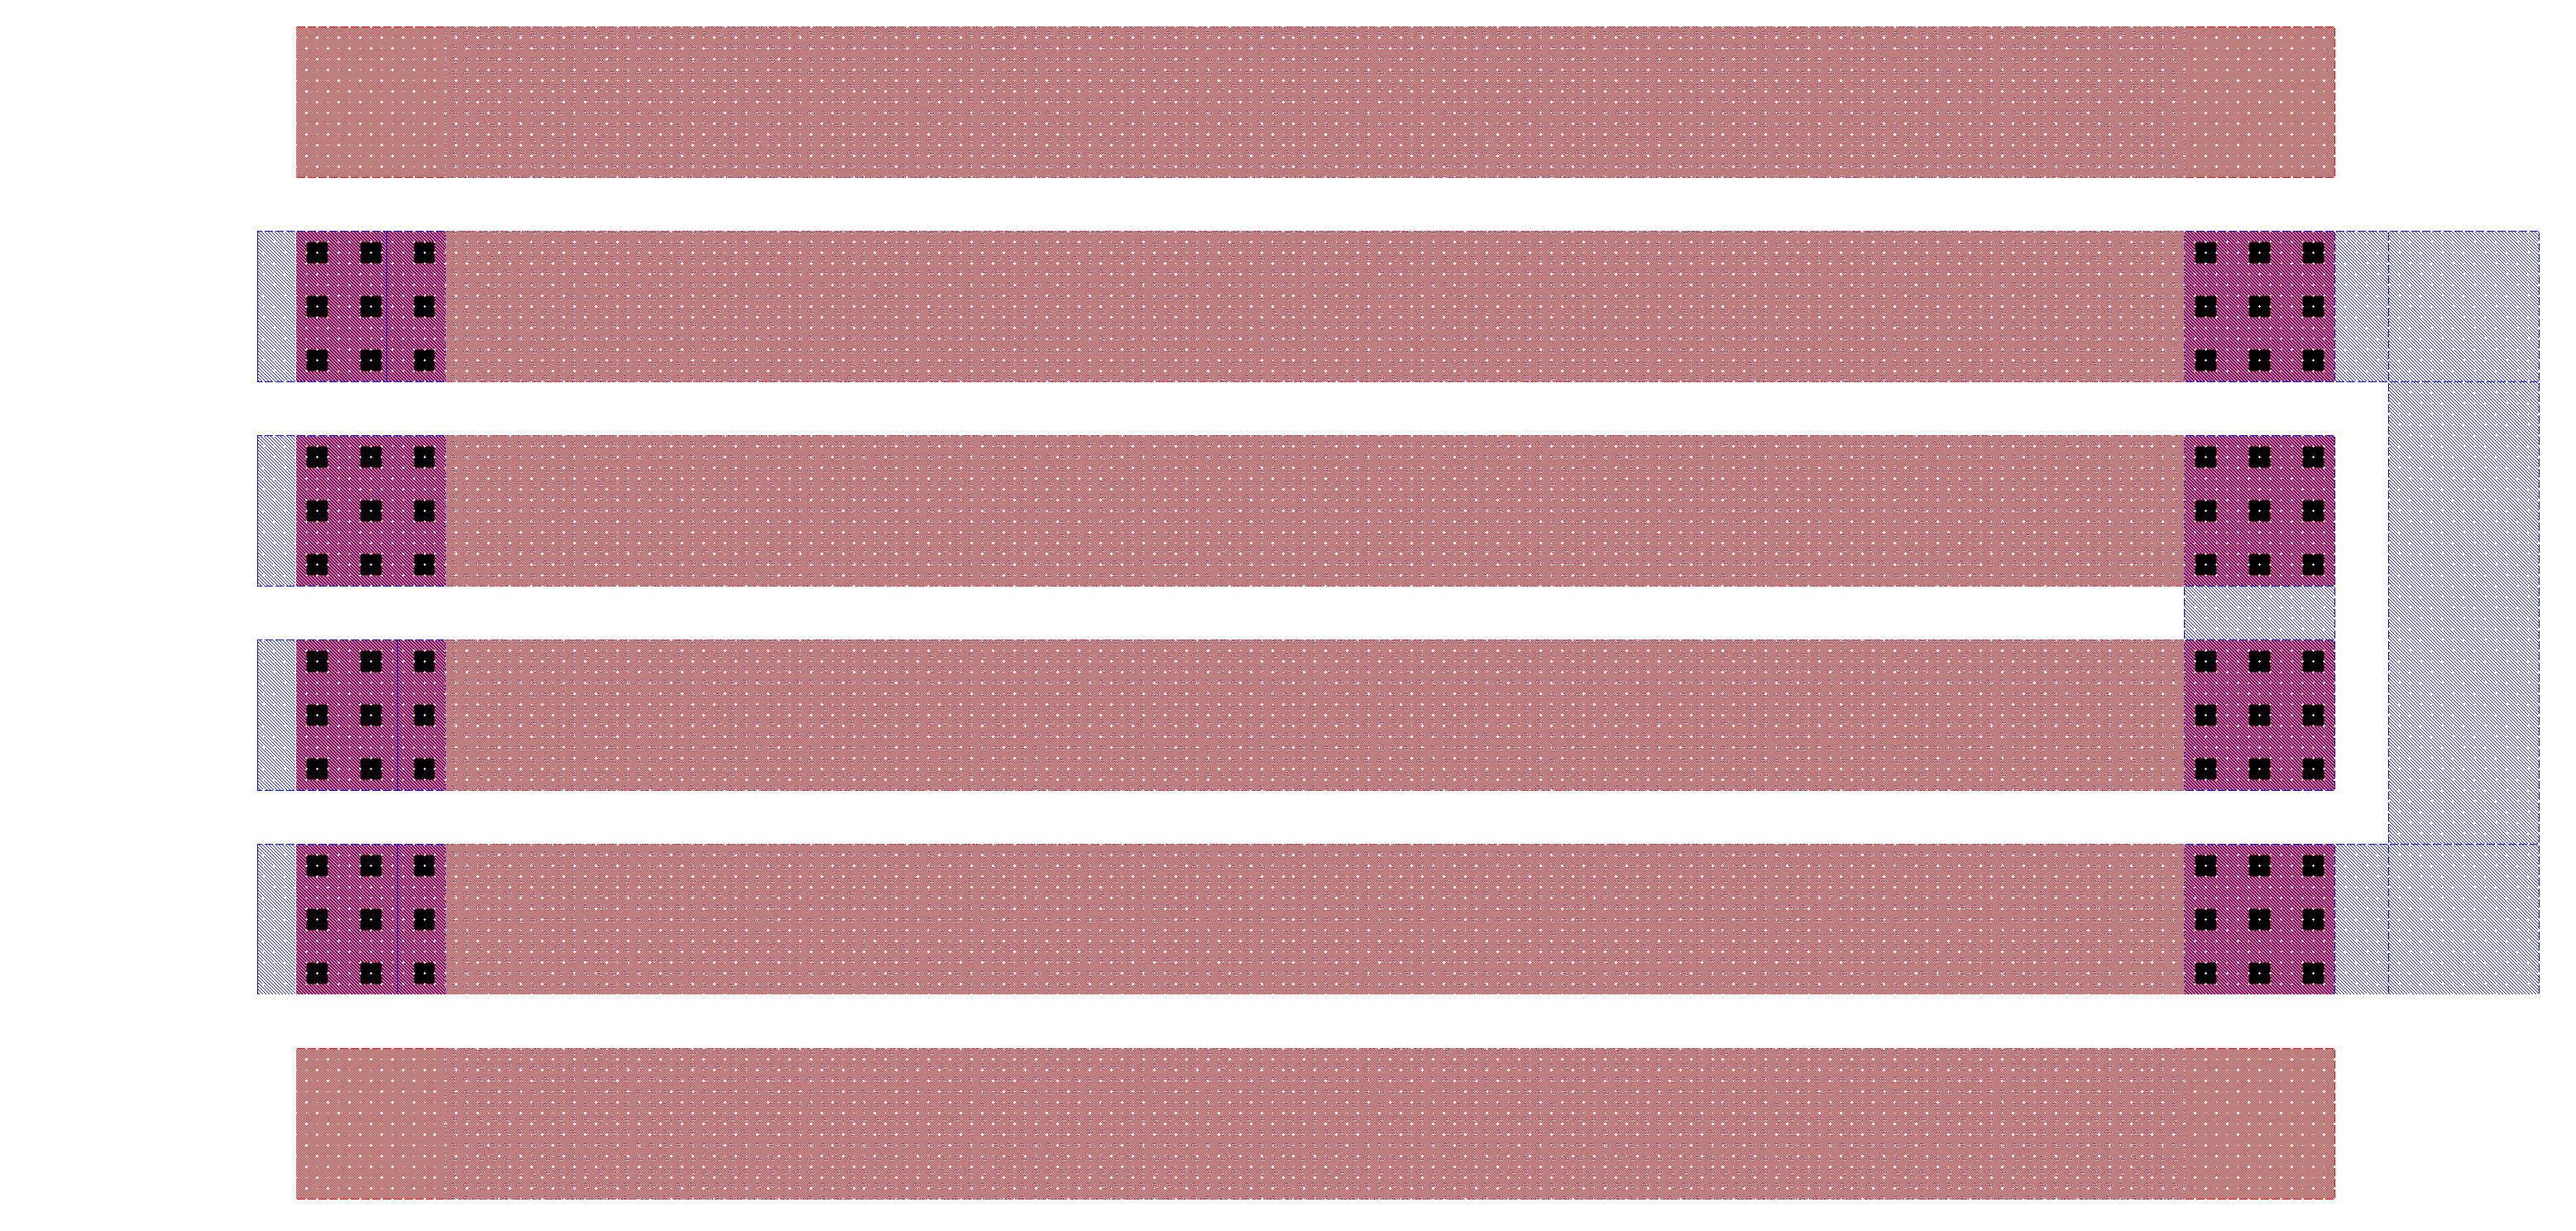
\includegraphics[width=0.6\textwidth]{L_RL}}
	\hfil
	\subfloat[$R_S$\label{subfig-1:L_RS}]
	{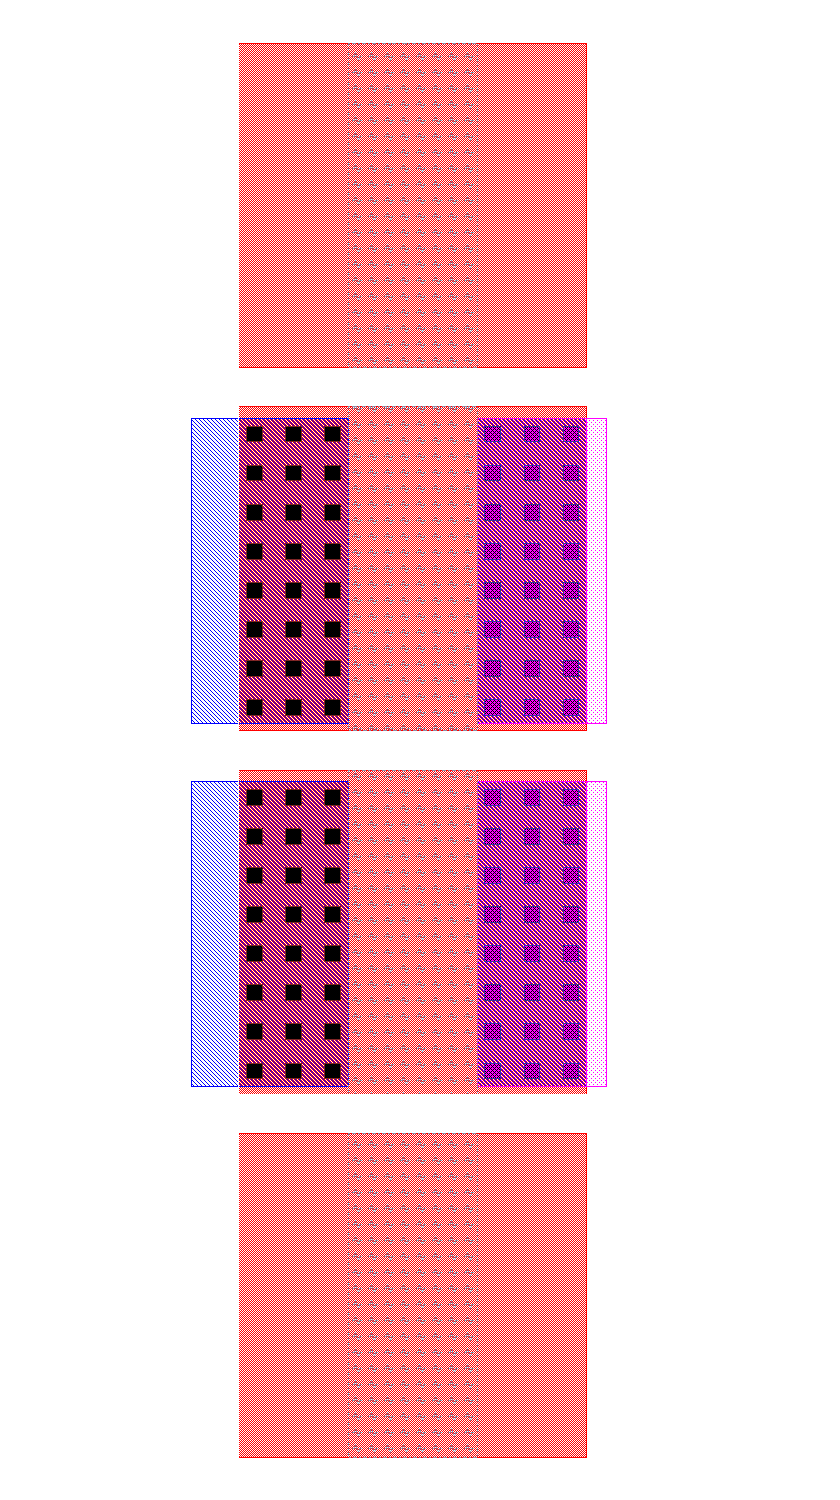
\includegraphics[width=0.15\textwidth]{L_RS}}
	\caption{Poly resistors layout}
\end{figure}

\subsection{Putting together the layout}
The layout has been organized in order to minimize the occupied surface area. The final configuration can be seen in figure \ref{L_complete_full}. 
\begin{figure}[H]
	\centering
	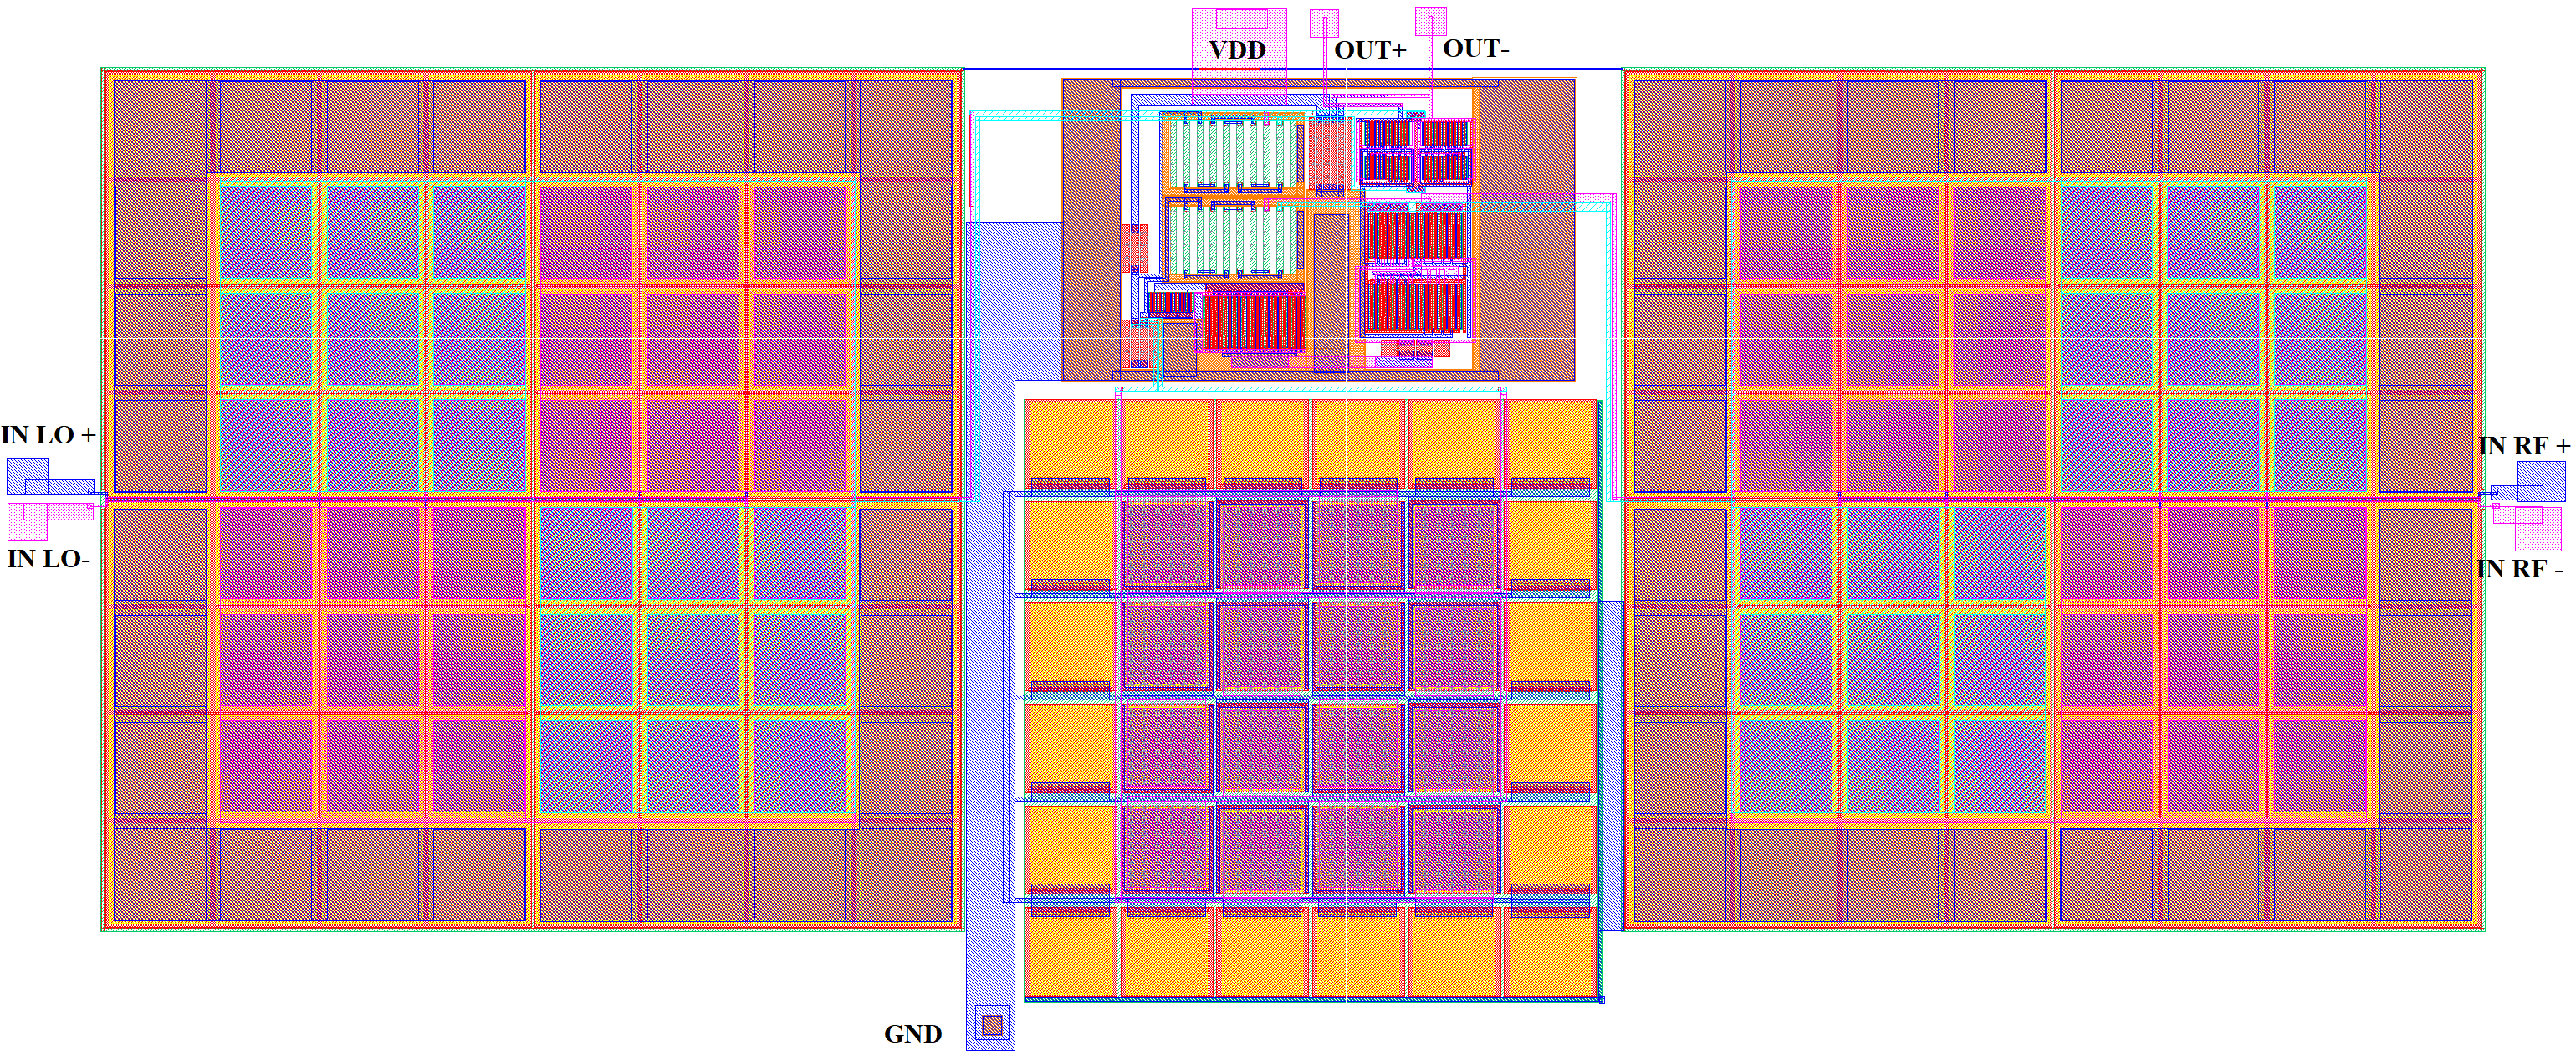
\includegraphics[width=1.1\textwidth]{L_complete_full}
	\caption{Layout of the complete Gilbert balanced mixer}
	\label{L_complete_full}
\end{figure}
Components have been placed to shorten interconnections, emphasize symmetries for matching and to make paths as equal as possible for high frequency signals.
Body contacts where placed all around the circuit where possible, and then connected to ground, in order captures free charges in the substrate reducing noise. A close up vision of the complete layout, without capacitors, is visible in figure \ref{L_complete_zoom}.

\begin{figure}[H]
	\centering
	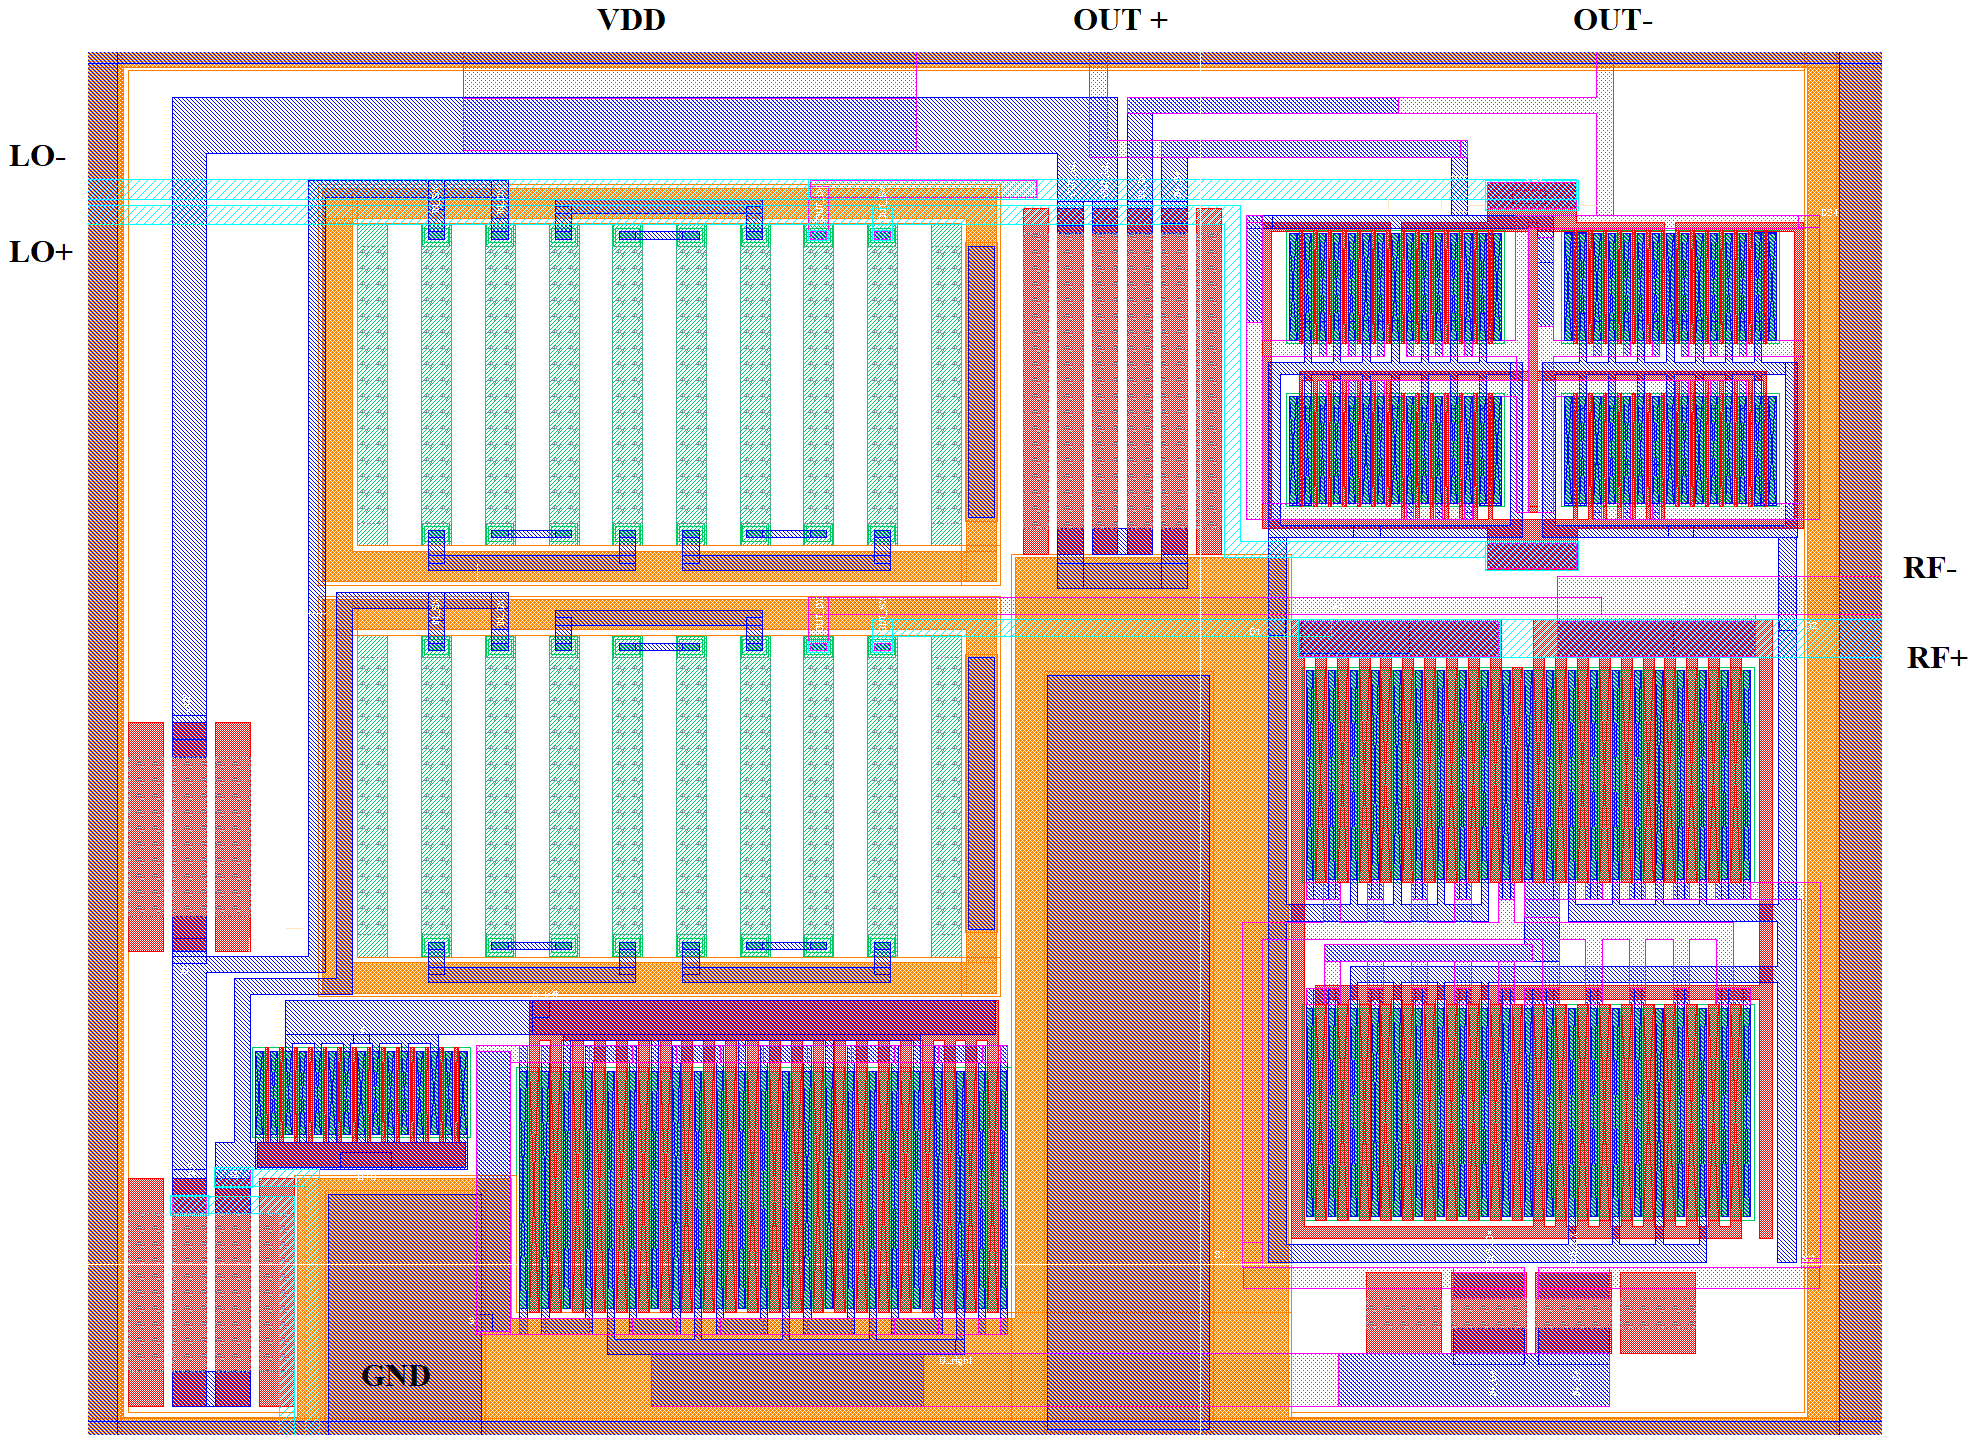
\includegraphics[width=1.05\textwidth]{L_complete_zoom}
	\caption{Close up of the complete layout}
	\label{L_complete_zoom}
\end{figure}

The whole occupied area is approximately \(0.7mm*1.8mm\) and it's mainly due to size of the signal capacitors. Such a big area can be also justified with the fact that the used technology is not the right one for this kind of RF design, and it was carried on mainly with the scope of learning how to layout a circuit.
